\chapter{Introduction to Graph Theory}

\begin{summary}
Informally, a graph is a picture with dots (we name them vertices)
connected by lines (edges).
They can often be used as an abstraction for solving a concrete
problem. They are a context in which many algorithms were (and are)
developed: shortest-path algorithms (think of GPS), spanning trees
(optimisation of networks), graph coloring (register allocation by
a compiler), maximal flow in networks, cycles of all kinds
\ldots Therefore, it pays off to formally study the abstract context of
graphs.

The next three chapters of this book formally deal with different kinds
of graphs and related concepts. In this chapter we first illustrate
the use of graphs for modelling and tackling various problems.

% The first part of this book deals with
% \begin{inparaenum}[]
% \item
% definitions related to graphs, and examples of some particular graphs,
% \item
% planar graphs - Euler's formula - $K_3$ and $K_{2,2}$ as minimal non-planar graphs,
% \item
% Eulerian and Hamiltonian cycles,
% \item
% weighted graphs,
% \item
% minimal spanning tree (Kruskal and Prim),
% \item
% a maximal flow algorithm and the SCCS algorithm,
% \item
% graph coloring,
% \item
% problem modeling with graphs.
% \end{inparaenum}
\end{summary}

%===============================================================================
\section{Three Coins}

Three coins are on a table heads (H) up, tails (T) down. You are
allowed to perform the following action as often as you want: flip any
two coins. Question: is it possible that after some actions, all
coins are tails up?

One way to solve this (type of) problem goes as follows: draw a graph
with each of the possible configurations of the 3 coins as a vertex,
and an edge between two vertices if the allowed action transform one
configuration into the other. We get the graph in Figure~\ref{munten}.

\begin{figure}[ht]
\begin{center}
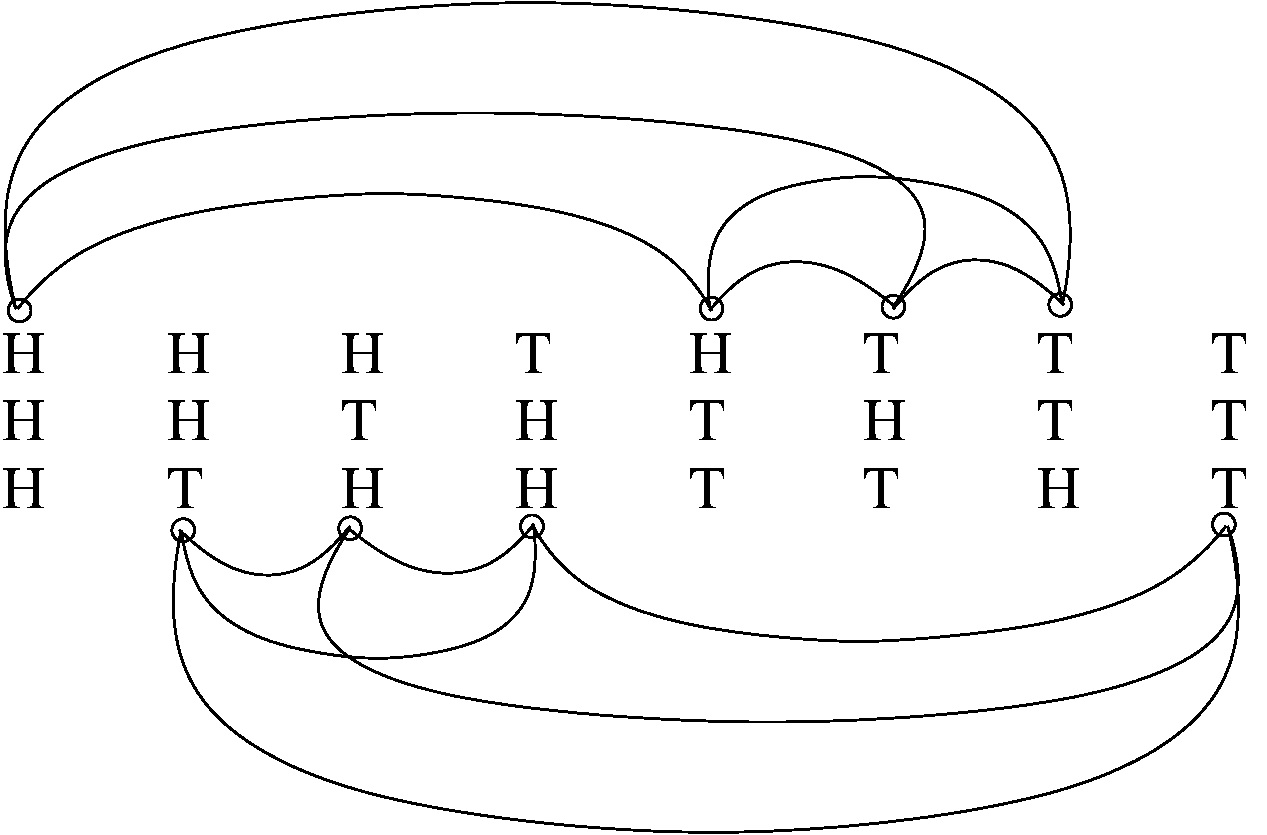
\includegraphics[width=0.5\linewidth,keepaspectratio]{munteneng}
\end{center}
\caption{The 3 coins graph \label{munten}}
\end{figure}

Just looking at the graph shows us that it is impossible to get from
the HHH configuration to the TTT configuration: they belong to a
different component of the graph. The property used here is {\em
reachability}.


%===============================================================================
\section{The Wolf, the Goat, the Cabbage, and the Farmer}

A farmer owns a wolf, a goat and a cabbage. He lives at the left bank
of a river, and he wants to move to the right bank. He also has a
small boat: it is too small to put all his belongings in it at the
same time, in fact, it is so small he can transport at most one
item at a time. He could transport his wolf, goat, and
cabbage to the right bank one by one, in some particular order, but the problem
is that when the wolf and the goat are left alone, the wolf will eat
the goat. Similarly for the goat and the cabbage: they can't be left
alone. So this simple plan does not work. Can the farmer transport all
his belongings to the other side so that nothing gets eaten?

You could of course try out all possibilities - why not try it now!
You notice that there is a problem of bookkeeping while doing that.
A better way is to note down all possible situations: a situation
describes who/what is on which side of the river, and is characterized
completely by what is on the left side. So, the situation FGC means
that the farmer, the goat and the cabbage are on the left bank, while
the wolf is at the right bank. Some situations - like GC - are a
priori forbidden. All situations can be described by the dots in
Figure~\ref{BWGK1}: we use $\ast$ to indicate that nothing is at the
left bank: it is the situation the farmer really wants.

\begin{figure}[ht]
\mbox{
\hspace{1cm}
\subfigure[All possible situations for the farmer, wolf, goat, and
cabbage]{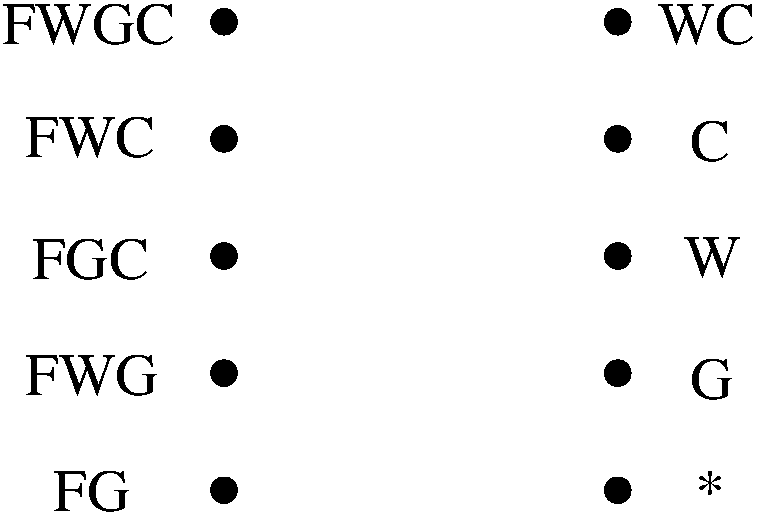
\includegraphics[height=0.12\textheight,keepaspectratio]{BWGK1eng} \label{BWGK1}}\hspace{2.5cm}
\subfigure[The graph describing the situations and their allowed
transitions]{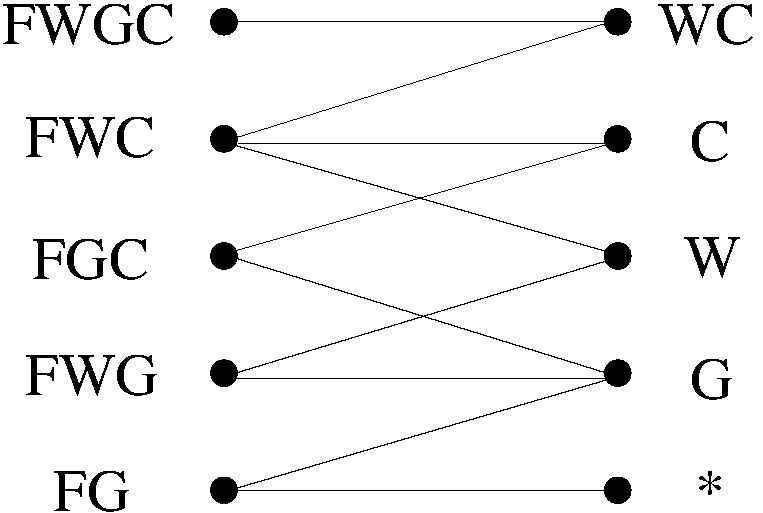
\includegraphics[height=0.12\textheight,keepaspectratio]{BWGK2eng} \label{BWGK2}
} }
\caption{The farmer, wolf, goat and cabbage problem}
\end{figure}

We can now connect any two situations $\alpha$ and $\beta$ if the
farmer can cross the river - possibly with one of his belongings - and
by doing so transforms $\alpha$ into $\beta$. We get the graph in
Figure~\ref{BWGK2}.  The problem is now reduced to the question: is
there a path from vertex FWGC to $\ast$ using the edges in
Figure~\ref{BWGK2}?

Again, reachability is the key concept, and the details of the problem
have been abstracted away.


%===============================================================================
\section{The Bridges of K\"onigsberg}

18$^{th}$ century, K\"onigsberg (now Kaliningrad in Russia): the river Pregel
crosses the city. It contains two islands, connected by a total of 7
bridges with each other and the river banks: see
Figure~\ref{pregel}. The citizens of K\"onigsberg used to make walks
during the weekend, and they wondered: is it possible to make a walk
(starting at home and arriving at home of course) so that every bridge
is crossed exactly once? They couldn't solve it. When the swiss
mathematician Leonhard Euler (1707-1783) visits the town, he hears
about the problem, solves it (negatively), and publishes the first
paper ever on graph theory.

\begin{figure}[ht]
\begin{center}
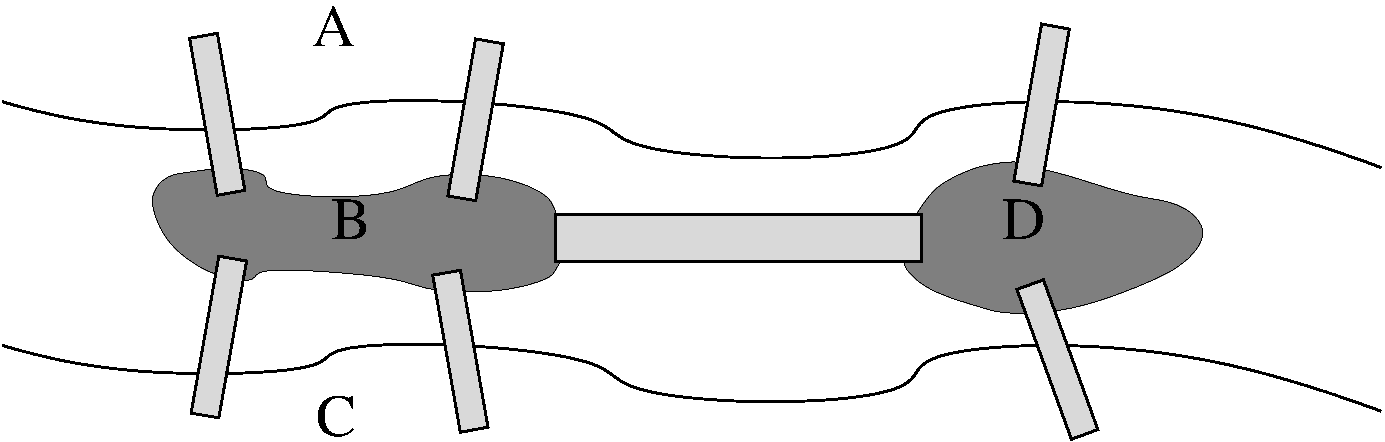
\includegraphics[width=0.4\linewidth,keepaspectratio]{pregel}
\end{center}
\caption{The bridges on the river Pregel \label{pregel}}
\end{figure}

How is this problem connected to graph theory? The graph
representation of the bridges and river banks can be seen in
Figure~\ref{pregelgraph}. The essence of the problem is now: does the
graph have a cycle (a closed path) that uses every edge exactly once?
This kind of cycle is now named an Eulerian cycle. We will later see
that the characterization of graphs with an Eulerian cycle is simple,
as well as finding an Eulerian cycle.

\begin{figure}[ht]
\begin{center}
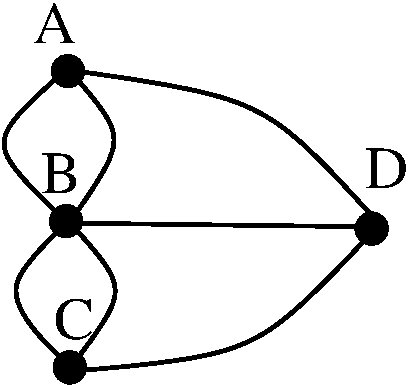
\includegraphics[width=0.15\linewidth,keepaspectratio]{pregelgraph}
\end{center}
\caption{The graph modeling the bridges over the Pregel \label{pregelgraph}}
\end{figure}

You might know the problem of finding an Eulerian cycle (or path) in a
different context: you are given a drawing in which points are
connected by lines; you are asked to draw it by putting your pen at
one point, never lifting it, following all lines not more than once.

Finding Eulerian cycles is important in real life: suppose you need to
check the state of the median strip of the highways. You need to
traverse all highways, but preferably only once.

%===============================================================================
\section{Hamilton's Toy}

Sir William Rowan Hamilton tried to commercialize circa 1850 a 3-D
puzzle in the form of a dodecahedron (it has 12 pentagons):
Figure~\ref{hamilton1} shows a planar representation of this spatial
object. Each corner had the name of a city and the problem consisted
in finding a closed path (a cycle) starting at a particular city so
that every city is visited exactly once. Such path is named a
Hamiltonian cycle. It turns out that finding such a cycle (or proving
it exists) is much more difficult than for Eulerian cycles.

\begin{figure}[ht]
\begin{center}
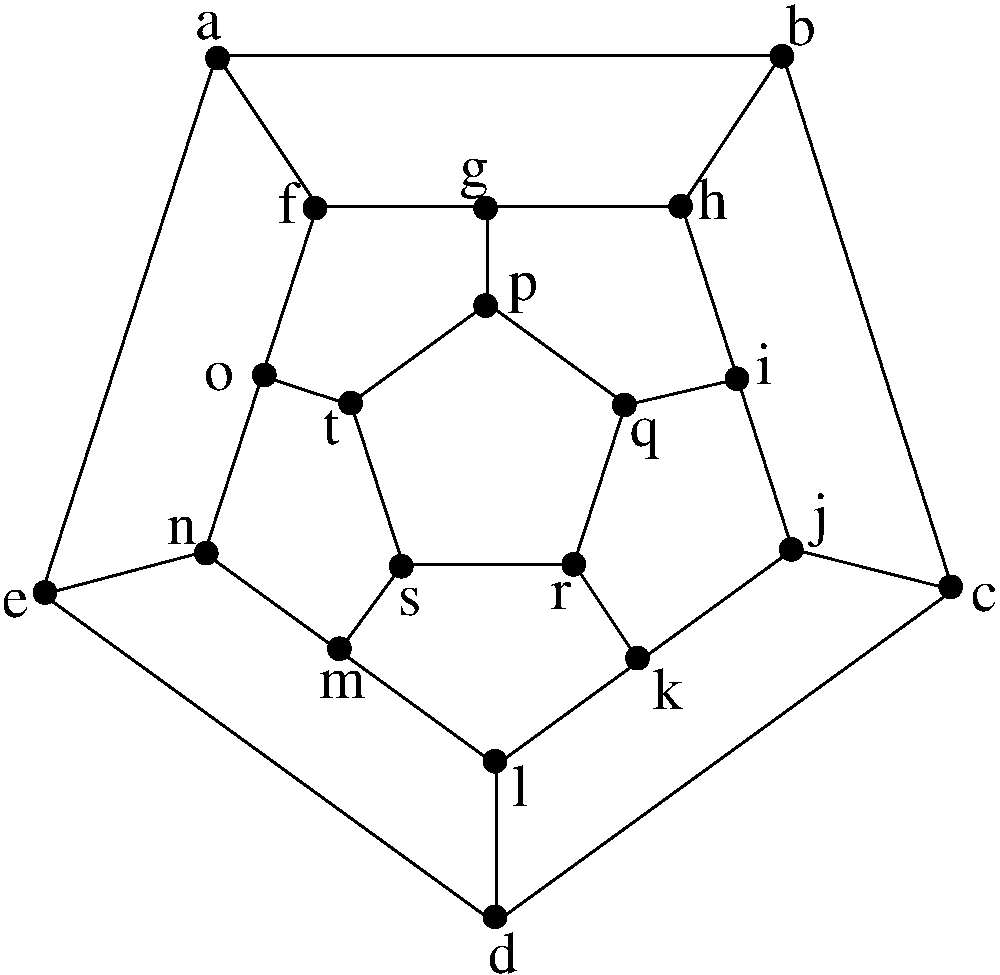
\includegraphics[width=0.4\linewidth,keepaspectratio]{hamilton}
\end{center}
\caption{Hamilton's puzzle
\label{hamilton1}}
\end{figure}

The puzzle was a commercial disaster, but it is at the heart of the
Travelling Salesman Problem.
The Postman Problem has a similar flavor: during his tour, a postman
wants to visit each street exactly twice (once at each side of the
street) \ldots is that always possible \ldots?

Figure~\ref{hamiltonkring} shows a Hamiltonian cycle for Hamilton's puzzle.

\begin{figure}[ht]
\begin{center}
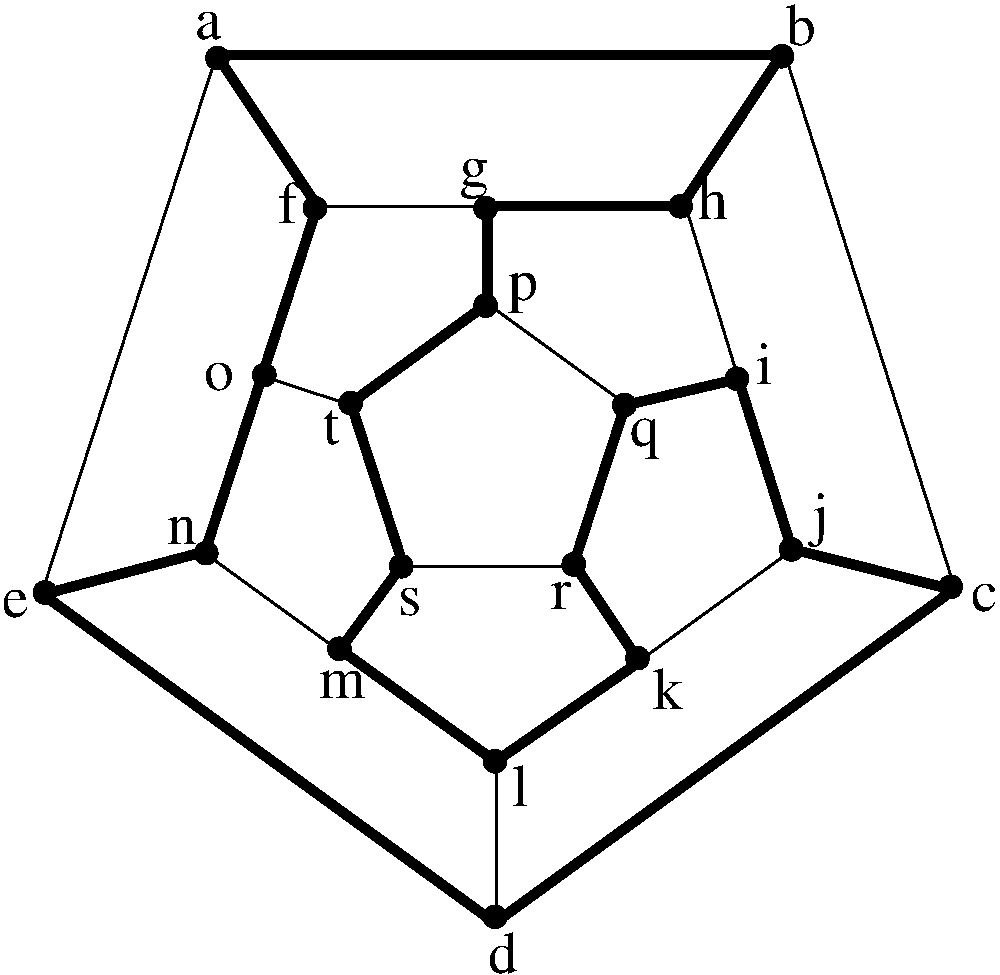
\includegraphics[width=0.6\linewidth,keepaspectratio]{hamiltonkring}
\end{center}
\caption{A solution for Hamilton's puzzle
\label{hamiltonkring}}
\end{figure}

%===============================================================================
\section{References}

\begin{itemize}
\item
Richard Johnsonbaugh ``Discrete Mathematics'', MacMillan, 1984
\item
Shimon Even ``Graph Algorithms'', Pitman, 1979
\item
Ralph P. Grimaldi ``Discrete and Combinatorial Mathematics''
\item
William Barnier, Jean B. Chan ``Discrete Mathematics''
\item
Michael Townsend ``Discrete Mathematics: Applied combinatorics and \\
graph theory''
\end{itemize}



%///////////////////////////////////////////////////////////////////////////////
\chapter{Graphs}

%===============================================================================
\section{Basic Definitions}

\begin{definition}[Graph]
A(n undirected) \textbf{graph} $G$ is a tuple $(V,E)$ in which
$V$ is a set of \textbf{vertices} and $E$ a (multi-)set
of \textbf{edges}; each edge $e \in E$ is an unordered pair $(v,w) \in
V \times V$; we write $e = (v,w)$ or $e = (w,v)$.
\end{definition}

We allow some freedom of notation and speech:
\begin{itemize}
\item
we write $G(V,E)$ for the graph $G$ with vertices $V$ and edges $E$
\item
we write $e \in G$ when $e \in E$ and $E$ is a subset of the edges of $G$
\item
we write $v \in G$ when $v \in V$ and $V$ is a subset of the vertices of $G$
\item
let the edge $e = (x,y)$, and $G(V,E)$, then $G \cup \{e\}$ denotes
the graph $(V \cup \{x,y\},E \cup \{e\})$; we say {\em add $e$ to $G$}
\item
let $b$ be a vertex, and $G(V,E)$, then $G \cup \{b\}$ denotes the
graph $(V \cup \{b\},E )$; we say {\em add $b$ to $G$}
\end{itemize}

We assume sometimes that the vertices are numbered from 1 to $n =
|V|$. We will deal only with finite graphs.

Edge is also used in the context of polyhedra, and that is no
surprise: the study of polyhedra and graphs have common points.

Note that $E$ can contain two edges $(v,w)$: we name those edges {\em
parallel}.

An edge $(v,w)$ is {\em incident on} the vertex $v$ (and on $w$);
the vertices $v$ and $w$ are {\em adjacent} to the edge $(v,w)$.

\begin{definition}[Directed graph (digraph)]
A directed \textbf{graph} $G$ is a tuple $(V,E)$ in which
$V$ is a set of \textbf{vertices} and $E$ a (multi-) set
of \textbf{edges}; each edge $e \in E$ is an ordered pair $(v,w) \in
V \times V$; we write $e = (v,w)$.
\end{definition}

You can think of a directed graph as a graph in which each edge has an
arrow, pointing from one vertex to the other.


\begin{definition}[Loop]
  \textup{A \textbf{loop} in a graph is an edge $(v,v)$. }
\end{definition}


\begin{definition}[Simple graph]
\textup{A graph is \textbf{simple} if the graph has neither parallel edges
nor loops.}
\end{definition}


\begin{definition}[Degree of a vertex]
  \textup{The \textbf{degree $\delta(v)$ of a vertex $v$} of graph
$(V,E)$ is the number of edges $(v,w) \in E$, where a loop counts for 2.}
\end{definition}


\begin{definition}[Isolated vertex or point]
A vertex $v$ in a graph $(V,E)$ is {\bf isolated} if $\delta(v)=0$.
\end{definition}


\begin{theorem}[Sum of vertex degrees] \label{somgraad}
The sum of all vertex degrees is even.
\end{theorem}
\begin{proof}
Since each edge $(v,w)$ contributes 1 to the degree of both $v$ as
$w$, each edge contributes 2 to the sum of all vertex degrees, hence
the conclusion.
\end{proof}


\begin{theorem}[Number of vertices with an odd degree]
The number of vertices with an odd degree is even.
\end{theorem}
\begin{proof}
Partition $V$ in the vertices with an even degree $\{a_i |
i=1,\ldots,n\}$, and the vertices with an odd degree $\{b_i |
i=1,\ldots,m\}$.  Then, because of Theorem~\ref{somgraad}
\[0 = \left(\sum_{i=1}^{n} \delta(a_{i}) + \sum_{i=1}^{m} \delta(b_{i})\right)
\bmod 2 = m \bmod 2 \] and the conclusion follows.  \end{proof}


\begin{definition}[Path]
\textup{A \textbf{path} (with length $n$) in a graph $(V,E)$ is a
sequence of edges
\[( e_1=(v_{1},v_{2}),\;e_2=(v_{2},v_{3}),\;\ldots, e_{n}=(v_{n},v_{n+1})).\]
We assume that it is clear which of the parallel edges is used (if at
all important). \\
In a simple graph, a path can also be characterized by a sequence of
vertices $(v_{1}, \ldots , v_{n+1})$}
\end{definition}

\begin{definition}[Simple path]
  \textup{A \textbf{simple path} $(v_{1}, \ldots , v_{n+1})$ is a path
  with the property that $\forall i,j: i \neq j \Rightarrow v_{i} \neq v_{j}$ }
\end{definition}



\begin{definition}[Cycle]
  \textup{A \textbf{cycle} is a path
    $((v_1,v_2),...,(v_n,v_{n+1}))$ such that all edges in it are
different and $v_{1} = v_{n+1}$.}
\end{definition}

A cycle is sometimes called a circuit.


\begin{definition}[Eulerian cycle (path)]
  \textup{An \textbf{Eulerian cycle (path)} is a cycle (path)
containing all edges exactly once.}
\end{definition}

\begin{definition}[Hamiltonian cycle]
  \textup{ A \textbf{Hamiltonian cycle} is a cycle containing all
vertices of the graph exactly once.}
\end{definition}


\begin{definition}[Connected graph]
  \textup{ A graph is \textbf{connected} if for every two different
vertices $v$ and $w$, there is a path from $v$ to $w$.}
\end{definition}



\begin{theorem}[Existence of an Eulerian cycle.]
A connected graph $G(V,E)$ has an Eulerian cycle if and only the degree of
each vertex is even.
\end{theorem}
The intuition behind the proof is that when you arrive in a vertex,
you can leave again because the degree is even. It therefore does not
matter which path you follow, as long as you don't return to the
starting point too soon. Even if you did, you can still mend the path.

\begin{proof}
~\\
\begin{itemize}
\item[\underline{$\Rightarrow$}:] In a connected graph with an Eulerian cycle, the cycle connects all
vertices as there is a path from each vertex to each other vertex and the cycle
covers all paths. While traversing the cycle, we leave every vertex in which we
arrive, and since all edges are traversed by the cycle, the degree of each
vertex is even.

\item[\underline{$\Leftarrow$}:] Construct a cycle $P$: start from any vertex $s$, follow any
edge incident on $s$; from then on extend the partial path with any
edge incident on the most recently added vertex, never using a
previously used edge. Repeat until there are no more edges to choose
from. Since the degree of each vertex is even, the just constructed
$P$ is a cycle starting in $s$ and arriving at $s$. If $P$ contains
all edges from $G$, the theorem is proven. Otherwise, there exists a
vertex $s'$ on the path $P$ from which an unused edge leaves (explain
why!). Construct a cycle $P'$ starting at $s'$ not using any edges
from $P$ (why is this possible?). Then add $P'$ to $P$: now you have a
larger cycle. One can repeat the procedure until there are no more
unused edges. Figure~\ref{euler4} illustrates the construction.
\end{itemize}
\begin{figure}[ht]
\begin{center}
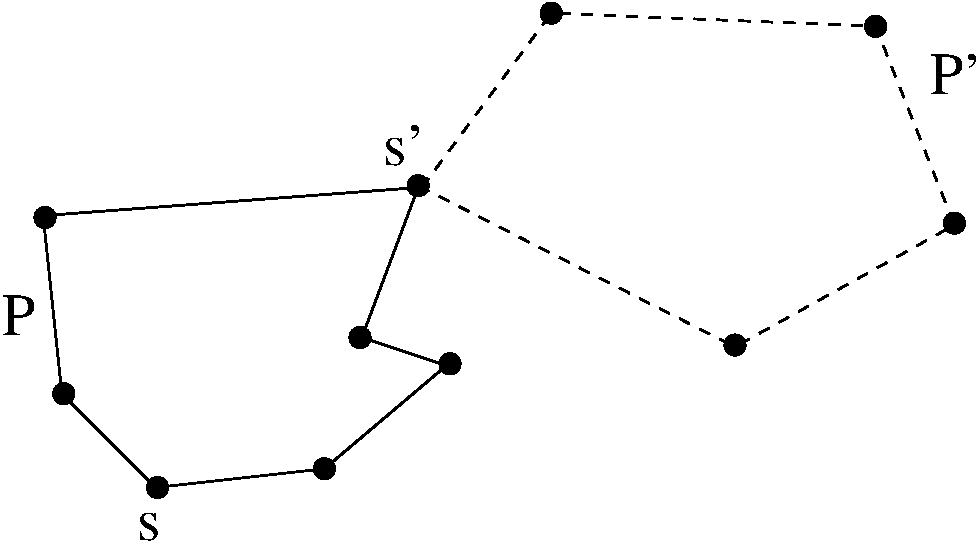
\includegraphics[width=0.4\linewidth,keepaspectratio]{euler4}
\end{center}
\caption{ $P$ and the extension $P'$ \label{euler4}}
\end{figure}
\end{proof}


\begin{theorem}[Existence of an Eulerian path]
  A connected graph $G$ has an Eulerian path from vertex $v$ to $w$
  ($v \neq w$) if $v$ and $w$ are the only vertices with an odd degree.
\end{theorem}
\begin{proof}
Consider the graph $G'$ obtained by adding the edge $(w,v)$ to $G$.
$G'$ is connected and each vertex has an even degree, so it has an
Eulerian cycle $(w,v,\ldots,w)$; delete the first edge from this cycle
to obtain the Eulerian path $(v,\ldots,w)$ in $G$.
\end{proof}

\begin{example}
Looking back at Figure~\ref{pregelgraph} (the graph modeling the
bridges in K\"onigsberg), you notice that there are four vertices with an
odd degree. It follows that there is neither an Eulerian cycle, nor an Eulerian
path.
\end{example}



\begin{definition}[Subgraph]
  \textup{A graph $(V_1,E_1)$ is a \textbf{subgraph} of $(V,E)$ if
    $V_1 \subseteq V$ and $E_1 \subseteq E$.}
\end{definition}



 \begin{definition}[Component of a  graph]
  \textup{A \textbf{component} $C$ of a graph $G$ is a maximal
    connected subgraph of $G$, i.e.
$\forall C' \subseteq G: C \subset C' \Rightarrow C'$ is not connected.}
\end{definition}

 \begin{theorem}[\label{partitie} Partition of a graph]
The components $(V_{i},E_{i})$ ($i=1,\ldots,n$) of a graph $(V,E)$
form a partition,
i.e. \\
$(V,E) = (\cup_{i=1}^{n} V_{i},\cup_{i=1}^{n} E_{i})$ and
for any $i \neq j$, $V_{i} \cap V_{j} = \emptyset$ and $E_{i} \cap E_{j} =
\emptyset$
\end{theorem}
\begin{proof}
Clearly every vertex and edge belongs to at least one component.
Suppose a vertex belongs to two components $\alpha$ and $\beta$, then
the union of $\alpha$ and $\beta$ is a connected subgraph of $(V,E)$
so $\alpha = \beta$, so $V_{i} \cap V_{j} = \emptyset$ for $i \neq
j$. Since an edge belongs to the component of its incident vertices,
the proof can be completed easily.
\end{proof}


Theorem~\ref{partitie} is important because it is often easier to
prove properties for connected graphs: Theorem~\ref{partitie} tells us
that a non-connected graph can be uniquely divided in connected
components.


%===============================================================================
\section{Graph Representations \label{voorstelgraph}}

Until now we have just drawn graphs. However, we often need a more
formal representation of graphs, e.g. because we need to write
programs dealing with graphs. There is no single best representation:
it depends on what we want to compute. So we introduce several
representations, first for undirected graphs, later for digraphs.

Let us number the $n = |V|$ vertices of $G(V,E)$ from 1 to
$n$. Construct an $n\times n$ matrix $A$ with $A(i,j)$ equal to 1 if
$(i,j) \in E$ and 0 otherwise. $A$ is called the adjacency matrix $G$:
it readily shows which vertices are adjacent.

\begin{figure}[ht]
\begin{center}
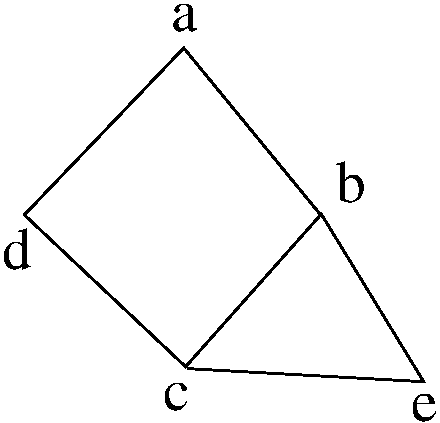
\includegraphics[width=0.15\linewidth,keepaspectratio]{adjacency1}
\end{center}
\caption{ Some graph \label{adjacency1}}
\end{figure}

\begin{example}
The adjacency matrix $A$ of the graph in Figure~\ref{adjacency1} is

\begin{center}
\mbox{\space \space \space}
$\begin{array}{ccccc}
a & b & c & d & e\\
\end{array}
$\\
$
\begin{array}{c}
a\\
b\\
c\\
d\\
e\\
\end{array}
$
$
\left(
\begin{array}{ccccc}
0 & 1 & 0 & 1 & 0\\
1 & 0 & 1 & 0 & 1\\
0 & 1 & 0 & 1 & 1\\
1 & 0 & 1 & 0 & 0\\
0 & 1 & 1 & 0 & 0\\
\end{array}
\right)
$
\end{center}
\end{example}

The adjacency matrix of a simple graph has only zeros on the main
diagonal. The adjacency matrix does not show whether a graph has
parallel edges. The adjacency matrix is symmetric and hence not a
very efficient representation of a graph. Still, it has interesting
properties.

\begin{example}
Compute $A^{2}$ for the example above. We get

\begin{center}
$
A^{2} = \left(
\begin{array}{ccccc}
2 & 0 & 2 & 0 & 1\\
0 & 3 & 1 & 2 & 1\\
2 & 1 & 3 & 0 & 1\\
0 & 2 & 0 & 2 & 1\\
1 & 1 & 1 & 1 & 2\\
\end{array}
\right)
$
\end{center}

We got the $(a,c)$ element of $A^{2}$ by:

\begin{center}
$
\left(
\begin{array}{ccccc}
0 & 1 & 0 & 1 & 0\\
\end{array}
\right)
\times
\left(
\begin{array}{c}
0\\
1\\
0\\
1\\
1\\
\end{array}
\right)
 =
0\times 0 + 1\times 1 + 0\times 0 + 1\times 1 + 0\times 1 = 2$
\end{center}

The positive contributions in the calculation result from the paths
$(a,b)-(b,c)$ and $(a,d)-(d,c)$. This shows that $A^{2}[i,j] = $ the
number of paths from vertex $i$ to vertex $j$ with length 2.
\end{example}
But we need to
be careful: the adjacency matrix does not show parallel edges, and
parallel edges increase the number of paths between two vertices.
As a consequence, the next theorem is about simple graphs.

 \begin{theorem}
\label{aantalpathen}
$ $ \\
Let $A$ be the adjacency matrix of a simple graph $G(V,E)$,\\
then
$A^{n}[i,j] = $ the number of paths with length $n$ from vertex $i$ to vertex
$j$.
\end{theorem}
\begin{proof} We use induction on $n$. For $n=1$, the theorem is true
because of the definition of adjacency matrix.

Suppose the theorem is true for $n$; we prove that the theorem is true
for $(n+1)$: $A^{n+1}=A^{n}*A$, so $A^{n+1}[i,j] = \sum_{k=1}^{\#V}
A^{n}[i,k]*A[k,j]$. By the induction hypothesis, $A^{n}[i,k]$ is the
number of paths from $i$ to $k$, and if there is an edge from $k$ to
$j$, (i.e. if $A[k,j] = 1$), then there are also $A^{n}[i,k]$ paths
from $i$ to $j$ passing through $k$ just before arriving at
$j$. Since no two paths are the same (why not?), the result for
$(n+1)$ follows.
\end{proof}

For the graph in Figure~\ref{adjacency1}, we have
\begin{center}
$A^{4} = \left(
\begin{array}{ccccc}
9 & 3 & 11& 1 & 6\\
3 & 15& 7 & 11& 8\\
11& 7 & 15& 3 & 8\\
1 & 11& 3 & 9 & 6\\
6 & 8 & 8 & 6 & 8\\
\end{array}
\right)
$
\end{center}

You can check manually that the theorem is true.

Making use of the previous result, we can derive that $(\sum_{k=1}^{n}
A^{k})[i,j]$ equals the number of paths from $i$ to $j$ and equal to
or shorter than $n$ edges.

The adjacency matrix can also be used in a different way: interpret
the numbers 0 and 1 as the boolean values $false$ and $true$, and
define boolean matrix multiplication as

\[(A*B)[i,j] = (A[i,1] \wedge B[1,j]) \vee (A[i,2] \wedge B[2,j]) \vee
\ldots \vee (A[i,n] \wedge B[n,j])\]


If $B$ is the boolean adjacency matrix of $G$, then $B^{n}[i,j]$
equals the truth value of the sentence {\em there exists a path of
length $n$ from $i$ to $j$}.

Analogously, $(\sum_{k=1}^{n} B^{k})[i,j]$ (sum means boolean sum,
i.e. $\vee$) is the truth value of {\em there exists a path from $i$
to $j$ of length smaller than or equal to $n$}.

For the usual adjacency matrix, the entries in this sum, for
successive values of $n$, grow indefinitely, but for the boolean
adjacency matrix, the entries can only be $false$ or $true$. Moreover,
they are monotonically increasing, so the limit exists. In fact, the
limit is reached after at most $|V|$ steps, and it is one way to
compute the transitive closure of the relation {\em is connected by an
edge}.

Another graph representation consists of the incidence matrix $I$: it
has a row for each vertex and a column for each edge. $I[i,j] = 1$
iff the $j^{th}$ edge is incident on $i$ and 0 otherwise.  The
incidence matrix of the graph in Figure~\ref{adjacency1} is

\begin{center}
\mbox{\space \space \space}
$\begin{array}{cccccc}
ab & ad & cd & bc & ce & be\\
\end{array}
$\\
$
\begin{array}{c}
a\\
b\\
c\\
d\\
e\\
\end{array}
$
$
\left(
\begin{array}{cccccc}
1 & \hspace{0.18cm} 1 & \hspace{0.18cm}0 & \hspace{0.18cm}0 & \hspace{0.18cm}0 & \hspace{0.18cm}0\\
1 & \hspace{0.18cm}0 & \hspace{0.18cm}0 & \hspace{0.18cm}1 & \hspace{0.18cm}0 & \hspace{0.18cm}1\\
0 & \hspace{0.18cm}0 & \hspace{0.18cm}1 & \hspace{0.18cm}1 & \hspace{0.18cm}1 & \hspace{0.18cm}0\\
0 & \hspace{0.18cm}1 & \hspace{0.18cm}1 & \hspace{0.18cm}0 & \hspace{0.18cm}0 & \hspace{0.18cm}0\\
0 & \hspace{0.18cm}0 & \hspace{0.18cm}0 & \hspace{0.18cm}0 & \hspace{0.18cm}1 & \hspace{0.18cm}1\\
\end{array}
\right)
$
\end{center}

The incidence matrix shows loops and parallel edges.

Instead of using an adjacency matrix, one can also use an {\em
adjacency list}: it is just a list of all edges.


The representation of digraphs can be done as for non-directed graphs:
the adjacency matrix has a 1 on the $(i,j)^{th}$ entry if there is a
directed edge from $i$ to $j$, and otherwise a 0. Usually, this matrix
is not symmetric, but since we never used that fact for non-directed
graphs, Theorem \ref{aantalpathen} applies also to digraphs, and the
idea of the boolean adjacency matrix does too.

One use of the boolean adjacency matrix is in finding out the
functions that are called (directly or indirectly) from a given
function in a given program: you can work that out yourself, and also
discover how you can detect {\em dead code} (compiler jargon),
i.e. functions that are not called by anyone. 
% In Section~\myref{sccs},
% this application example is used in an interesting graph algorithm.


%===============================================================================
\section{Graph Isomorphisms}

We do the following experiment: all of you take a pen and paper, and
without looking at what your neighbour is doing, you follow the
following instructions:

\begin{itemize}
\item[]
- draw 5 points and put a name next to each of them \\
- connect the first point you drew with the second point\\
- connect the second with the third\\
- connect the third with the fourth\\
- connect the fourth with the fifth\\
- connect the fifth with the first\\
\end{itemize}

There is a chance that some students come up with one of the graphs in
Figure~\ref{experiment1}.

\begin{figure}[ht]
\begin{center}
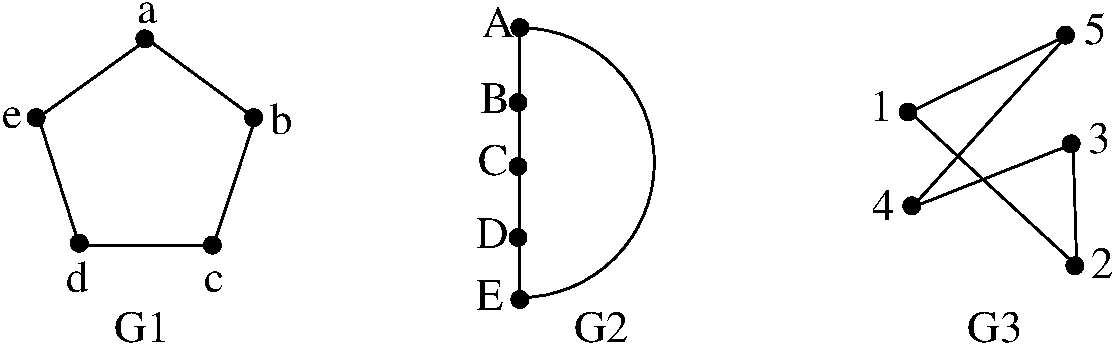
\includegraphics[width=0.6\linewidth,keepaspectratio]{experiment1}
\end{center}
\caption{Three different graphs, or are they equal?\label{experiment1}}
\end{figure}

All these graphs look different, but they were drawn following the
same instructions: there is a good reason for considering them {\em
the same} in some sense, hence the following definition:

\begin{definition}[Graph Isomorphism]\label{isomorfegraphs}
\textup{The graphs $G_{i}(V_{i},E_{i})$ (i = 1,2) are
    \textbf{isomorphic}, if there exists a bijection $f: V_{1}
\rightarrow V_{2}$ such that $g: E_{1} \rightarrow E_{2}$ specified by
$g((v,w)) = (f(v),f(w))$ for all $v,w \in E_{1}$ is well defined,
i.e. $g((v,w)) \in E_{2}$ and a bijection.  Such $f$ is named a
graph isomorphism.}
\end{definition}

Between $G1$ and $G2$ of Figure~\ref{experiment1}, there exists
the isomorphism $f$:
\begin{itemize}
\item[]
f(a) = B\\
f(b) = C\\
f(c) = D\\
f(d) = E\\
f(e) = A
\end{itemize}

You can check that this is a graph isomorphism between $G_{1}$ and
$G_{2}$. Another characterisation of isomorphic graphs relies on the
following theorem:

\begin{theorem}[Characterisation of isomorphic graphs with
the incidence matrix]
Graphs $G_{1}$ and $G_{2}$ are isomorphic if and only if there is an
ordering of the vertices and edges so that the incidence matrices of
$G_{1}$ and $G_{2}$ are equal.
\end{theorem}
\begin{proof}
~\\
\begin{itemize}
\item
Let $G_{1}$ and $G_{2}$ be isomorphic, with isomorphism $f$.
Choose any order of the vertices of $G_{1}$. Now order the vertices of
$G_{2}$ by: $f(v) < f(w) \Leftrightarrow v < w$; the order on the
edges of $G_{2}$ is induced in the same way by any order on the edges
of $G_{1}$ and the bijection on the edges. The incidence matrices are
equal.
\item If the incidence matrices are equal, the isomorphism $f$ is
trivial to specify.
\end{itemize}
\end{proof}

We know that the adjacency matrix does not fully determine a graph,
since parallel edges and loops are not visible in the adjacency
matrix. Consequently the following theorem is limited to simple
graphs.

\begin{theorem}[Characterisation of isomorphic simple graphs
with the adjacency matrix]
The simple graphs $G_{1}$ and $G_{2}$ are isomorphic if and only if
there is an ordering of the vertices so that the adjacency matrices of
$G_{1}$ and $G_{2}$ are equal.
\end{theorem}

\begin{proof} Please prove this yourself.
\end{proof}

The theorems on graph isomorphism provide algorithms using the
concrete representation of the graphs. However, every currently known
algorithm for testing whether two graphs are isomorphic is at least
exponential. On the other hand, there exist very efficient tests that
can show that two graphs are {\em not} isomorphic: one checks whether
some graph properties that are {\em invariant} under graph isomorphism
hold for both graphs. Such properties can be based on the number of
vertices, the number of edges, the degrees of the vertices \ldots We will
later see more of such properties. But remember that these simple
tests never tell you that two graphs are isomorphic, only that two
graphs are not isomorphic.



%===============================================================================
\section{Weighted Graphs}

 \begin{definition}[Weighted graph]
  \textup{ A \textbf{weighted graph} $(V,E)$ is a graph in which each
edge $e \in E$ has a \textbf{weight $w(e)$} $\in \R^{+}_0$. The
weight $w(G)$ of a weighted graph $G$, is the sum of the weights of
all the edges of $G$.  }
\end{definition}

The weight of an edge can be interpreted as the length of an
edge, or some cost associated with the use of the edge in a path: if
the graph models a road network, then the weight can be a distance
between cities, or a toll to be paid to use the road. The {\em weight
of a path} is the sum of the weights of the edges in the path. It is
clear that in the case of road networks, one would be naturally
interested in minimal weight paths connecting two given nodes, or put
differently, one is interested in {\em shortest} paths. Since two such
nodes are necessarily in the same component, this section deals with
connected graphs.

The {\em existence} of a shortest path in a connected (and finite)
graph is easy to prove (do it anyway). We are now interested in {\em
constructing} a shortest path. We restrict ourselves to simple graphs:
loops can't occur in a shortest path, and of the parallel edges
between two nodes, we need only the shortest one.

% Algorithms in this chapter consist of a sequence of instructions,
% numbered 1,2, \ldots . At the end of instruction $n$, there is an
% implicit {\bf Go to instruction $n+1$}. {\em Stop} means the algorithm
% finishes.


%===============================================================================
\section{Planar Graphs}

Informally, a planar graph is a graph one can draw on a sheet of
paper so that no two edges cross: there is no need for the third
dimension to achieve this non-crossing. There is a formal definition
as well: look it up. We will use the informal definition in proofs.

Another important class of graphs is the class of {\em bipartite}
graphs.

 \begin{definition}[Bipartite graph]
  \textup{A \textbf{bipartite graph} is a graph $(V,E)$ with $V =
V_{1} \cup V_{2}$ so that $V_{1} \cap V_{2} = \emptyset$ and $E
\subseteq V_{1} \times V_{2}$ }
\end{definition}

In words: in a bipartite graph, one can identify two disjoint subsets
of vertices, so that all the edges have an element of each subset as
an endpoint (and consequently, there are no edges that connect nodes
from the same subset).

Figure~\ref{kuratowski1} shows one such graph at the right.

$K_{n,m}$ denotes the bipartite graph in which $|V_{1}| = n$ and
$|V_{2}| = m$, and such that every vertex in $V_{1}$ is connected to
every vertex of $V_{2}$. $K_{n,m}$ occurs naturally when one considers
the problem of connecting $n$ houses with $m$ utilities (water, gas,
electricity, internet \ldots).

$K_{n}$ denotes the graph with $n$ vertices, in which there is an edge
between every two vertex. Such graphs are {\em completely
connected}, and we name them cliques.

The $K$ is in honour of Kazimierz Kuratowski, a famous graph theorist.

Figure~\ref{kuratowski1} shows $K_{4}$ and $K_{2,2}$.

\begin{figure}[ht]
\begin{center}
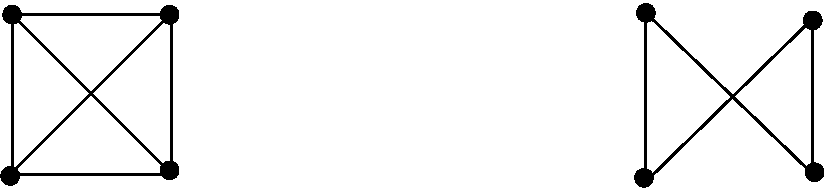
\includegraphics[width=0.4\linewidth,keepaspectratio]{kuratowski1}
\end{center}
\caption{$K_{4}$ and $K_{2,2}$ \label{kuratowski1}}
\end{figure}

When you try drawing $K_{n}$ on paper for successive values of $n$,
and such that no two edges cross, you notice that from $n=5$ on, it is
no longer possible. Similarly, trying this for successive values of
$(n,m)$ and $K_{n,m}$, it fails for all $n,m > 2$.

As we said before, graphs one can draw in the plane without crossing
edges are named \textbf{planar}. As an application: if the graph of a
road network is planar, there is no need for tunnels or bridges. Euler
proved the following formula in 1752\footnote{Descartes
($\pm$ 1600) knew the formula and most probably so did Archimedes
($\pm$ --250).}:

 \begin{theorem}[Euler's formula for planar graphs]
If $G$ is a connected planar graph with $e$ edges, $v$ vertices and
$f$ {\em faces} then $v-e+f = 2$.
\end{theorem}

We haven't defined a face yet: informally, it is a piece of the plane
enclosed by a minimal cycle. The infinite part of the plane
that lies outside of a (drawing of a) graph also counts as a face. The
origin of the word {\em face} is in the study of polyhedra.


\begin{proof} We use induction on the number of edges. Suppose
$e=1$. Then $G$ is one of the graphs in Figure~\ref{euler1}. In
both cases, the Euler's formula is correct.  Suppose the formula is
correct for all graphs with $n$ edges. Let $G$ be a graph with $(n+1)$
edges.

\begin{figure}[ht]
\begin{center}
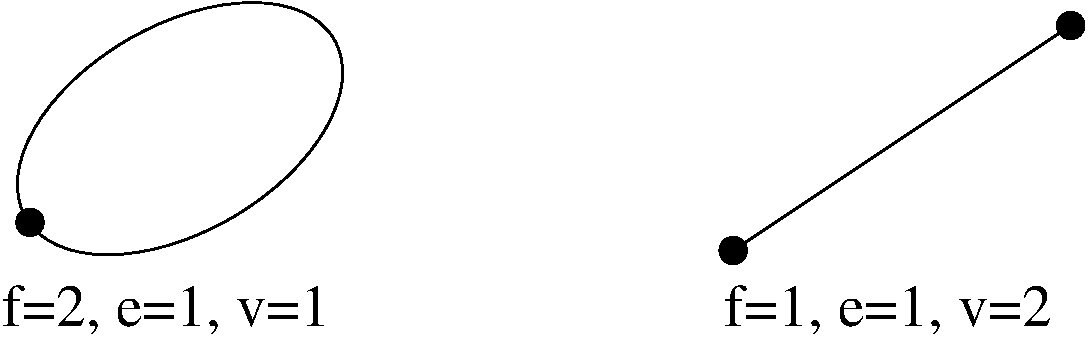
\includegraphics[width=0.4\linewidth,keepaspectratio]{euler1}
\end{center}
\caption{The two graphs with $e=1$ \label{euler1}}
\end{figure}

1) First assume that $G$ does not contain a cycle. Consider a maximal
simple path in $G$; that path contains a vertex $a$ with $\delta(a) =
1$: now consider the graph $G'$ which you obtain by removing from $G$
the vertex $a$ and the only edge arriving there; $G'$ has 1 vertex
and 1 edge less than $G$, the same number of faces, and $G'$ is also
connected (why?), so Euler's formula is valid for $G'$, and
consequently also for $G$ (see e.g. Figure~\ref{euler2}).\\
\begin{figure}[ht]
\begin{center}
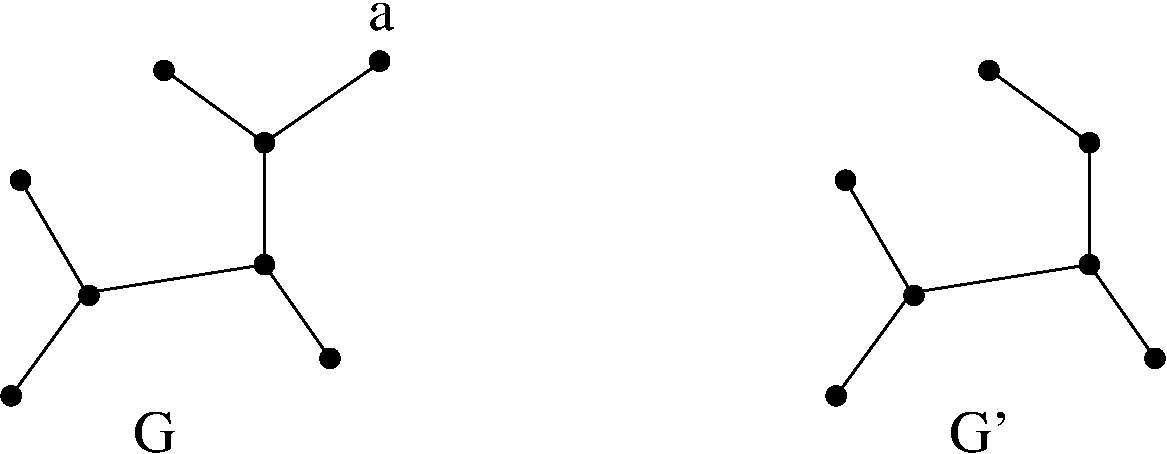
\includegraphics[width=0.4\linewidth,keepaspectratio]{euler2}
\end{center}
\caption{G without a cycle \label{euler2}}
\end{figure}

2) Suppose now that $G$ contains a cycle: take away any edge $x$ from
this cycle, but not its endpoints; the result is $G'$ (see
e.g. Figure~\ref{euler3}).
\begin{figure}[ht]
\begin{center}
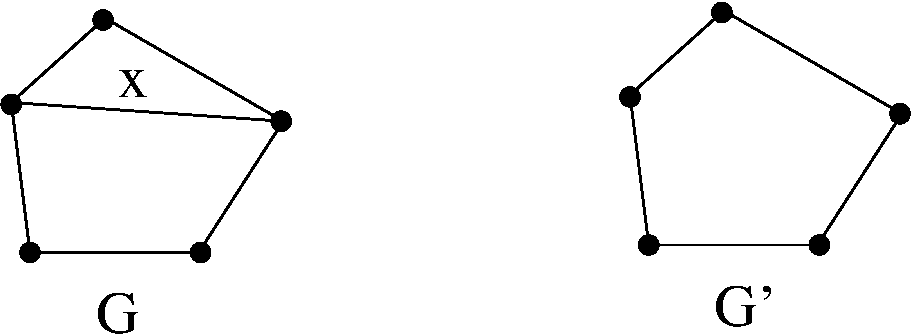
\includegraphics[width=0.4\linewidth,keepaspectratio]{euler3}
\end{center}
\caption{$G$ with a cycle \label{euler3}}
\end{figure}
$G'$ has $n$ edges, the same number of vertices as $G$, and one less
face than $G$; $G'$ is connected (why?); so Euler's formula is valid
for $G'$ (by the induction hypothesis), and it follows that Euler's
formula is also valid for $G$.
\end{proof}

Note that the connectedness condition is essential: the graph with two
vertices and no edge, has $f = 1, e = 0, v = 2$, so Euler's formula is
not valid. You should be able to generalize Euler's formula to
non-connected graphs, taking into account the number of components.

The origin of Euler's interest in this formula lies in the study of
spatial objects, more specifically polyhedra. This interest
existed already since Greek ancient history: regular polyhedra were
supposed to be the building blocks of the world. The formula expresses
the relation between the number of faces, edges and vertices of a
polyhedron. The transformation from a polyhedron and a planar graph
can be visualised as follows: imagine the polyhedron is drawn on a
balloon. Carefully make a hole in the middle of any face, and stretch
the hole until all the material is in a plane. The resulting picture
of edges and vertices form a planar graph. The face that was punctured
corresponds to the infinite face.

 \begin{theorem}
$K_{3,3}$ and $K_{5}$ are not planar.
\end{theorem}
\begin{proof}
Suppose $K_{3,3}$ is a planar graph. Let $\beta$ be the total number
of edges in all faces: an edge counts $n$ times if that edge occurs in
$n$ faces. Since (in a planar drawing) every edge can belong to at most 2
faces, we know that $2*e \geq \beta$.

Moreover, every cycle in $K_{3,3}$ has at least 4 edges (why?) from
which it follows that $\beta \geq 4*f$. Together with the previous
inequality, we derive $e \geq 2*f$. Now use Euler's formula to
eliminate $f$ from the right hand side. We get $e \geq 2*(e-v+2)$.
Fill out the values for $e$ and $v$ for $K_{3,3}$, and get $9 \geq
10$, which is not true. So $K_{3,3}$ is not planar.

Every cycle in $K_{5}$ has minimally 3 edges \ldots\ and the rest of
the proof is like above.
\end{proof}


When two graphs are isomorphic, they are basically the same up to a
renaming of the vertices. But graphs sometimes look similar even
though they they do not have the same number of edges or
vertices. E.g. if we add a vertex in the middle of an edge, it feels
like nothing essential has changed in the graph. For one thing, its
planarity has not changed, neither its connectivity (and you may
perhaps think of other properties that remain invariant). The
operation of adding the extra vertex is named subdivision or expansion
of the graph. The inverse operation is named {\em smoothing (out)} the
graph. The latter consists of replacing two edges $(a,b)$ and $(b,c)$
of which $\delta(b) = 2$ by one edge $(a,c)$. See Figure~\ref{rij1}.



\begin{figure}[ht]
\begin{center}
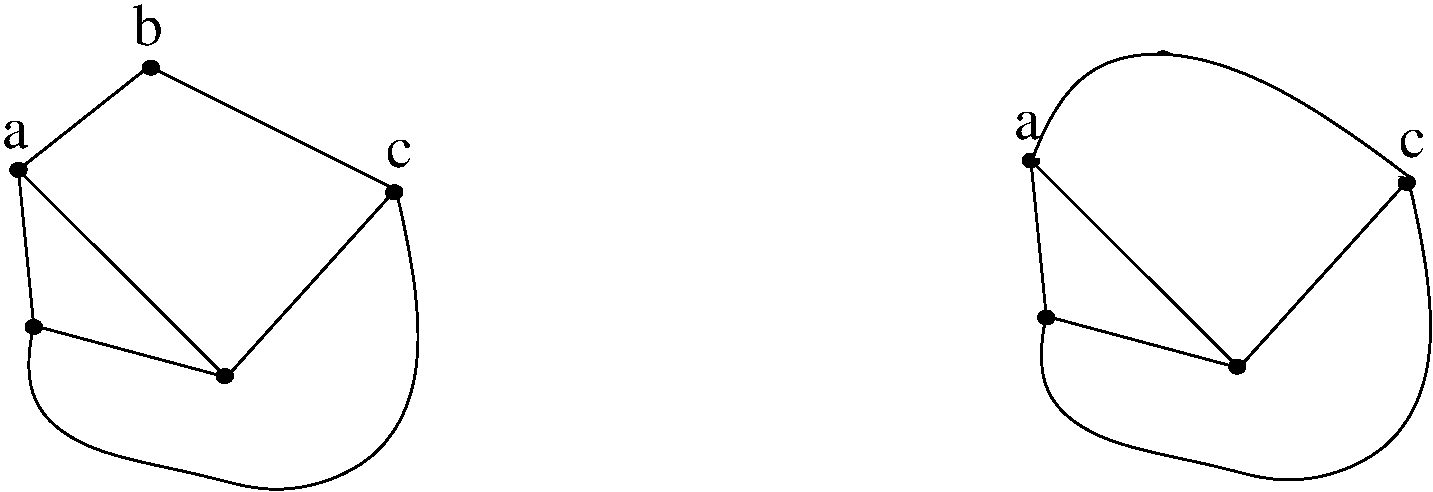
\includegraphics[width=0.4\linewidth,keepaspectratio]{rij1}
\end{center}
\caption{Smoothing a graph \label{rij1}}
\end{figure}

\begin{definition}
  \textup{Two graphs $G_{1}$ and $G_{2}$ are \textbf{homeomorphic} if
by applying smoothing to both graphs, one obtains isomorphic graphs.}
\end{definition}

 \begin{theorem}[Kuratowski's Theorem]
A graph is planar if and only if it does not contain a subgraph
homeomorphic to $K_{5}$ nor $K_{3,3}$.
\end{theorem}
\begin{proof}
One direction is obvious (but please give arguments!). The other direction
is out of the scope of this course.
\end{proof}

The above theorem basically says that $K_{5}$ and $K_{3,3}$ are in
some sense the smallest non-planar graphs.


%===============================================================================
\section{Graph Coloring}

 \begin{definition}
\textup{A \textbf{coloring} of a graph $(V,E)$ is an assignment of a
  color to each $v \in V$ such that the colors of $v$ and $w$ differ
  if $(v,w) \in E$. An
  \mbox{\textbf{n-coloring}} is a coloring with $n$ or less
  (different) colors. A \textbf{minimal} coloring is an $n$-coloring
  with minimal $n$.}
\end{definition}

There are lots of practical applications of (minimal) graph colorings.
Just a few examples:

\begin{itemize}
\item
Suppose you need to plan 4 meetings, involving persons A,B,C and D. The
first meeting must be attended by A and B; the second by A and C; the
third by B, C and D, and the fourth one by C and D. What is the
minimal number of time slots you can make all these meetings happen?
You may assume you have enough meeting places, and that each meeting
takes the same time. Of course, a person can't attend two meetings at
the same time.

You can represent this problem by the graph in Figure~
\ref{planning1}: each vertex corresponds to a meeting, and two
meetings are connected if they can't be at the same moment (because
some person needs to attend both). Now find a minimal coloring of this
graph, et voil\`{a}! Each color corresponds to a new time slot.
\begin{figure}[ht]
\begin{center}
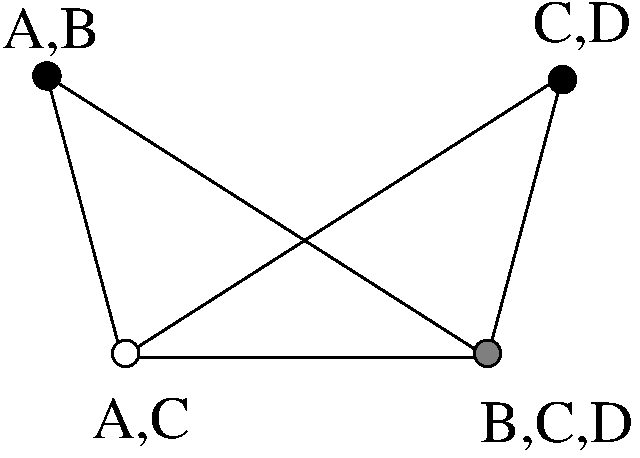
\includegraphics[width=0.2\linewidth,keepaspectratio]{planning1}
\end{center}
\caption{The meeting graph with a minimal coloring\label{planning1}}
\end{figure}

\item
You need to organize the goods in a supermarket on the racks, but some
goods can not be put next to each other, e.g. fuel can't be next to
bread, porn not next to cleaning powder, etc. Once more, you can
construct a graph representing the constraints, and a coloring of the
graph solves your problem.

\item
A compiler tries to put integer variables in machine registers
instead of in memory (why?). There are typically more variables than
available registers, but the same register can be used for more than
one variable. For example, consider the following code:


\parbox{9cm}{
\begin{tabbing}
123 \= 1234 \= 12 \= 12 \= 12 \kill
\> \> \{\\
\> \> \> int i,j,k,l,m;\\
\\
\> \> \> i = 1;\\
\> \> \> j = 2;\\
\> \> \> k = i+j;\\
\> \> \> i = 3;\\
\> \> \> j = 4;\\
\> \> \> l = i+j;\\
\> \> \> m = k+l;\\
\> \> \}
\end{tabbing}
}\\

$i$ and $l$ can be assigned the same register, and likewise for $k$
and $m$. You can find that out by constructing the inference graph of
this piece of code: the graph has the variables as vertices, and an
edge between two variables whose value is {\em alive} at the same
moment. Figure~\ref{regalloc1} shows the corresponding graph.

\begin{figure}[ht]
\begin{center}
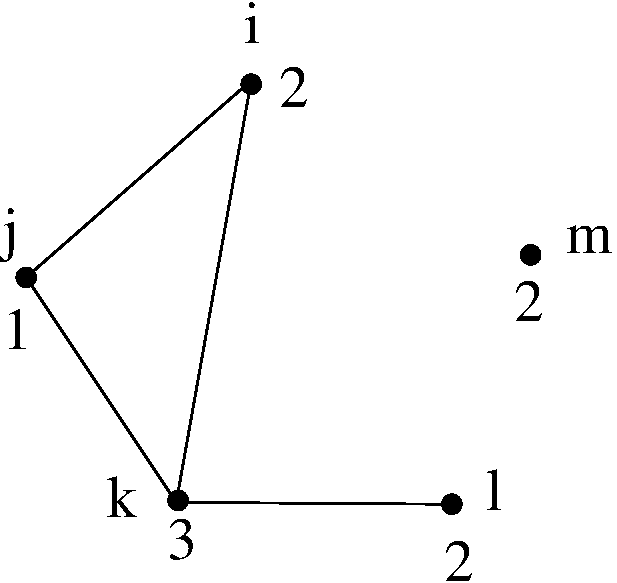
\includegraphics[width=0.2\linewidth,keepaspectratio]{regalloc1}
\end{center}
\caption{The interference graph and a coloring (with numbers) \label{regalloc1}}
\end{figure}

A minimal coloring determines the minimal number of registers needed
to assign each variable in a register, and also an optimal assignment.

\end{itemize}

A problem with practical implications, and historically important, is
the 4-color problem: is it possible to color each map with four
colors, so that no two neighboring countries have the same color? This
problem was set up by Francis Guthrie around 1850, and conjectured to
have a positive answer. Despite several attempts, the conjecture
remained unproven until 1976: K. Appel and W. Haken proved that there
exist 1936 graphs of which at least one must be in any 4-colorable
graph, and then proved that such graphs are not minimal ... The proof
was performed by a computer program.

The connection between map coloring and graph coloring is rather easy
for planar graphs. A map is a planar graph $G$, and can be turned into
another planar graph - its {\em dual} - $G'$ as follows: assume for
the sake of simplicity that each region in the map is a country. Each
country has a capital inside that country. Now construct the graph
with the capitals as nodes, and define an edge between two capitals if
their countries share a border. Figure~\ref{dual1} shows some
examples.


\begin{figure}[ht]
\begin{center}
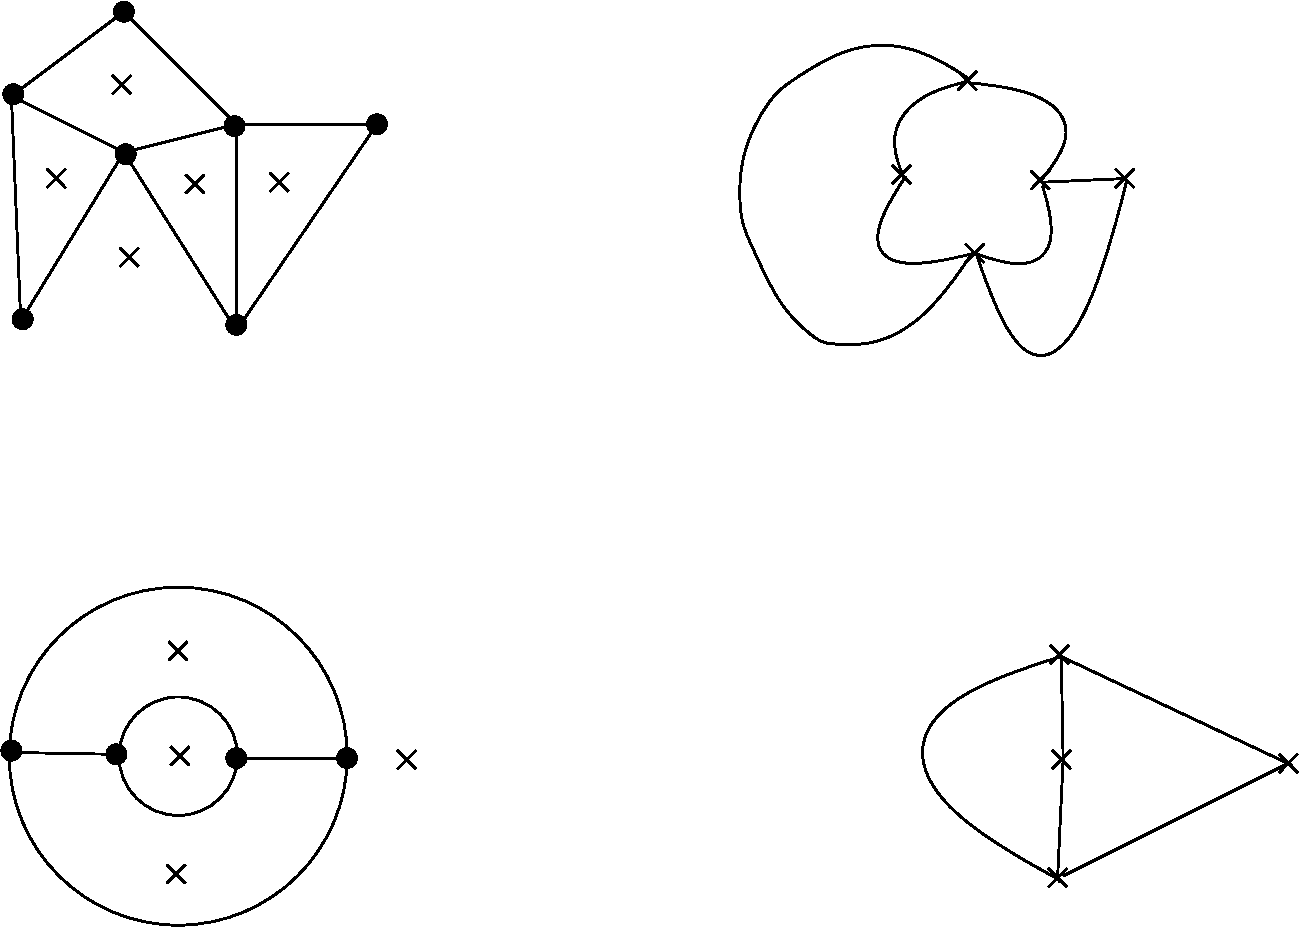
\includegraphics[width=0.6\linewidth,keepaspectratio]{dual1}
\end{center}
\caption{Two planar maps and their dual graphs\label{dual1}}
\end{figure}

Note that the dual graph of a planar map is planar, and simple. A
coloring of the dual graph, corresponds to a coloring of the map - and
vice versa.

In the rest of this section, we prove the 5-color theorem: every
planar graph can be colored with 5 colors.

 \begin{theorem} $e \leq 3*v-6$ for every planar, simple graph
     $G$ with more than one edge.\label{euler}
\end{theorem}
\begin{proof}
We prove the theorem only for connected graphs: first remove
every vertex from $G$ with a degree of 1 (and the corresponding edge),
until no more such vertices exist. The resulting graph $G'$ is still
planar, simple and connected. Denote the number of its edges by $e'$,
the number of its vertices by $v'$; the number of faces is $f$
because removing the particular edges did not change that. So we have
$e-e'=v-v'$ which is equal to the number of removed edges (or
vertices). Denote that quantity by $t$. We now make a case distinction:

1) if $e' = 0$ then $v' = 1$; since $e > 1$ we also have $t > 1$;
so we know: $e = t$ and $3*v-6 = 3*(v'+t) -6 = 3*t-3$; since $t \leq
3*t-3$, we get $e \leq 3*v-6$.

2) $e'$ can't be equal to 1 or 2 (why not?)

3) $e' > 2$; every face is delimited by at least 3 edges (because
there are no loops or parallel edges); let $\sum$ denote the sum of
the number of edges in all faces. then $\sum \geq 3*f$; since each
edge borders exactly 2 faces (why?), we also have $\sum = 2*e'$, so
$2*e' \geq 3*f$. Now use Euler's formula for $G'$ to eliminate $f$
from this inequality, and you get: $e' \leq 3*v'-6$ and thus $e'+t
\leq 3*(v'+t)-6$ and $e \leq 3*v-6$.
\end{proof}

 \begin{theorem} A planar, simple graph has at least one
 vertex - say $v$ - with $\delta(v) \leq 5$.
\end{theorem}
\begin{proof}
This is clearly true for graphs with 1 or 2 vertices. Suppose the
theorem is not true for a certain graph with at least 3 vertices,
i.e. this graph has degree at least 6 for each vertex. Then the sum of
the degrees of all the vertices is at least $6*v$, so, $e \geq 3*v$,
in contradiction with the $e \leq 3*v-6$ from the previous theorem.
\end{proof}

We are now ready to state and prove

 \begin{theorem} 5 colors is enough to color any simple,
     planar graph $G(V,E)$.
\end{theorem} % uit Townsend
\begin{proof} (the proof follows Townsend)

We use induction of the number of vertices: a $G$ with just one vertex,
can clearly be colored with 5 colors. Also, assume $G$ is connected:
if not, the theorem will be proven true for its components, and carry
over to the whole graph. So, assume that the theorem is true for
graphs with $n$ vertices; let $G$ have $n+1$ vertices. Then there is
at least one vertex $v$ with degree 5 or less.

1) If $v$ has degree 4 or less, then $v$ occurs in $G$ as in
Figure~\ref{5kleuring1}.

\begin{figure}[ht]
\begin{center}
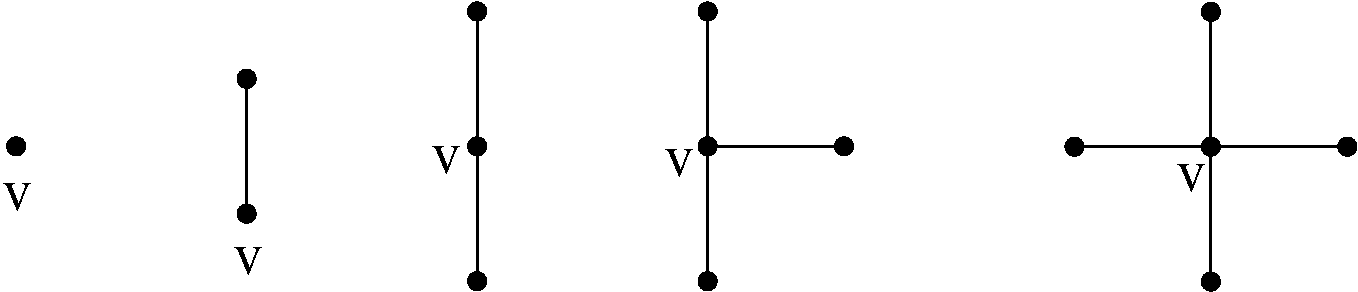
\includegraphics[width=0.6\linewidth,keepaspectratio]{5kleuring1}
\end{center}
\caption{The 5 possibilities in which $\delta(v) < 5$ \label{5kleuring1}}
\end{figure}

Consider the $G'$ obtained by deleting $v$ from $G$ (and the edges
arriving in $v$). $G'$ has the required properties for the theorem,
and it has only $n$ vertices, so by the induction hypothesis, it has a
$5$-coloring. Since $v$ has at most 4 neighbors, $v$ can get a color
different from the color of all its neighbors, resulting in a
$5$-coloring of $G$.

2) If $\delta(v) = 5$, then $v$ occurs in $G$ as in
Figure~\ref{5kleuring2}: each neighbor $w_{i}$ of $v$ has a color
$c_{i}$ ($i = 1,\ldots,5$) as obtained by a $5$-coloring of $G'$.

\begin{figure}[ht]
\begin{center}
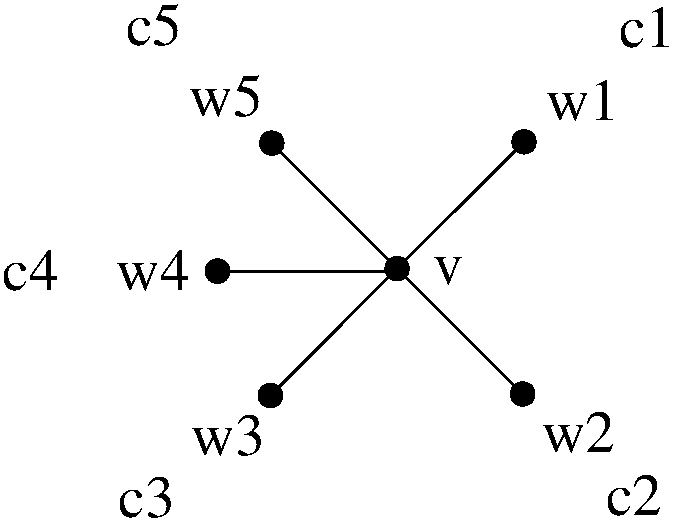
\includegraphics[width=0.25\linewidth,keepaspectratio]{5kleuring2}
\end{center}
\caption{$\delta(v) = 5$ \label{5kleuring2}}
\end{figure}

We still need to determine a color for $v$. If the neighbors of $v$ do
not use all 5 colors, we can give $v$ any remaining color.

So, assume that all five $c_{i}$ are different. Consider the set
$P_{1,3}$ of all paths in $G'$ starting at $w_{1}$ and whose vertices
have alternating colors $c_{1}$ and $c_{3}$. We name such paths
$c_{1}-c_{3}$ paths.  There are two possibilities:

\begin{description}
\item[$P_{1,3}$ does not contain a path that contains $w_{3}$:]
  for each vertex in the paths $P_{1,3}$, change color $c_{1}$ in
  $c_{3}$ and vice versa. We obtain a different $5$-coloring of $G'$
  (why?) and now vertices $w_{3}$ and $w_{1}$ have the same color
  $c_{3}$, so $v$ has no neighbor with color $c_{1}$. This means the
  new 5-coloring of $G'$ can be extended to a $5$-coloring of $G$, by
  assigning $v$ the color $c_{1}$.

\item[$P_{1,3}$ contains a path $p_{1,3}$ that contains $w_{3}$:]
  construct the path set $P_{2,5}$; as you can see in
  Figure~\ref{5kleuring3}, $P_{2,5}$ cannot contain a path that
  contains $w_{5}$; indeed, if such a path $p_{2,5}$ exists, then both
  $p_{1,3}$ and $p_{2,5}$ can be extended with the vertex $v$ so that
  they form cycles in $G$; these cycles must intersect, but not in a
  vertex, because of the different colors. But we have started from a
  plane drawing of the graph, so no intersection is possible. This
  means that no path in $P_{2,5}$ arrives at $w_{5}$, and we can use
  the trick.
\end{description}

\begin{figure}[ht]
\begin{center}
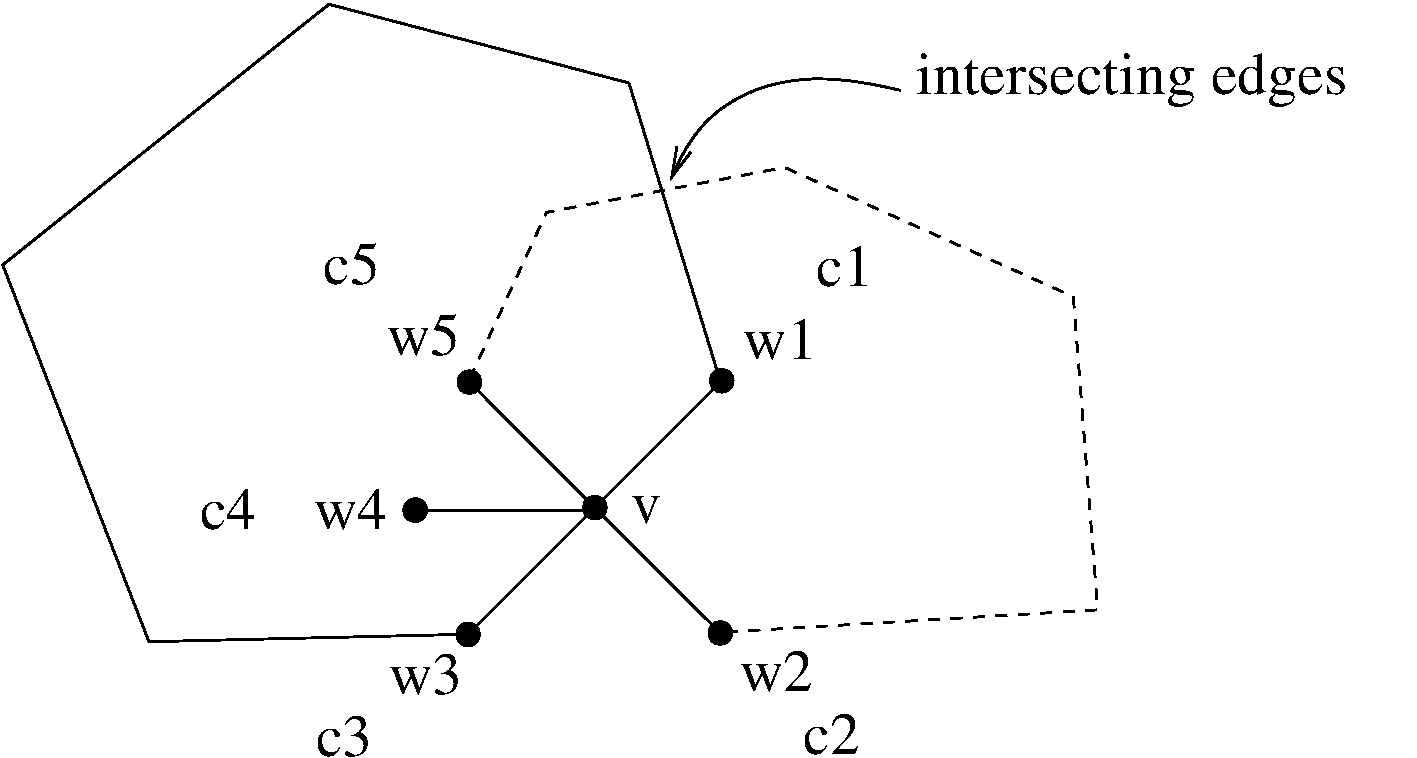
\includegraphics[width=0.4\linewidth,keepaspectratio]{5kleuring3eng}
\end{center}
\caption{$p_{1,3}$ and $p_{2,5}$ \label{5kleuring3}}
\end{figure}
\end{proof}

Appel and Haken {\em proved} that every planar graph has a
$4$-coloring, so they {\em proved} the 4-color conjecture for planar
maps.

This is a good moment to reflect on the concept of a {\em computer
  proof}. Whether something is accepted as a proof or not, is mainly a
social given. It feels true that the mathematical correctness of a
proof is independent of people agreeing with it, but a proof exists
mainly by the grace of the community accepting the proof, even if the
proof turns out to be incorrect later. So it is up to the community
(only to the mathematical community?) to accept or reject computer
proofs: one could imagine a branch of science that accepts only hand
written proofs on paper, just as there is a branch of mathematics that
accepts only constructive proofs, and no existential proofs. It is not
possible to decide unequivocally whether to accept computer proofs just
based on scientific arguments. But the fact is that the more proofs are
only possible by computer, the more we are inclined to accept such
proofs, especially if the theorems so proven have useful consequences.

One could argue that it is in principle possible to check a computer
proof by hand, or prove (by hand) that the computer program generating
the proof is correct. That is currently not possible for larger
programs. Moreover, one would also have to prove the correctness of
the machine executing the program \ldots something we might want to
leave to another computer program?

Returning to the coloring of graphs: there are non-planar graphs with
no 4-coloring, e.g. $K_{n}$ with $n > 4$ needs at least $n$ colors,
and the same holds for graphs containing the clique $K_n$. But there also
exist graphs not containing $K_4$ (or larger) with no
3-coloring. Finally, lots of non-planar graphs have a 4-coloring. More
specifically, every bipartite graph (e.g. $K_{3,3}$) has a 2-coloring.


% %===============================================================================
% \section{Strongly Connected Components}\label{sccs}
% 
% We abbreviate {\em strongly connected component} to SCC. Robert Endre
% Tarjan \footnote{Turing award 1986} - the master algorithmist -
% designed a very nice algorithm in 1972 that partitions the vertices of
% a digraph into SCCs. An SCC is a (maximal) set of vertices in which
% every node is connected to every other node of the same set. We first
% look at an application. Below is a program in pseudo-code, from which
% everything is stripped except the procedure call and definitions.
% 
% \begin{Verbatim}[frame=single, samepage=true, fontsize=\scriptsize]
% main()               venus()                aurochs()           tarpan()
% {                    {                      {                   {
%   venus();             pluto();               dodo();             aurochs();
%   aurochs();           venus();               tarpan();         }
% }                    }                      }
% 
%                      pluto()                dodo()              mamoet()
%                      {                      {                   {
%                        venus();               tarpan();           mamoet();
%                      }                        mamoet();         }
%                                             }
% \end{Verbatim}
% The {\em call graph} of this program can be seen in
% Figure~\ref{vbtarjan}: the vertices are the procedures; there is a
% directed edge $(p_1,p_2)$ if and only if $p_1$ calls $p_2$. We have
% left out the self-calls.
% 
% 
% 
% \begin{figure}[h]
% \begin{center}
% 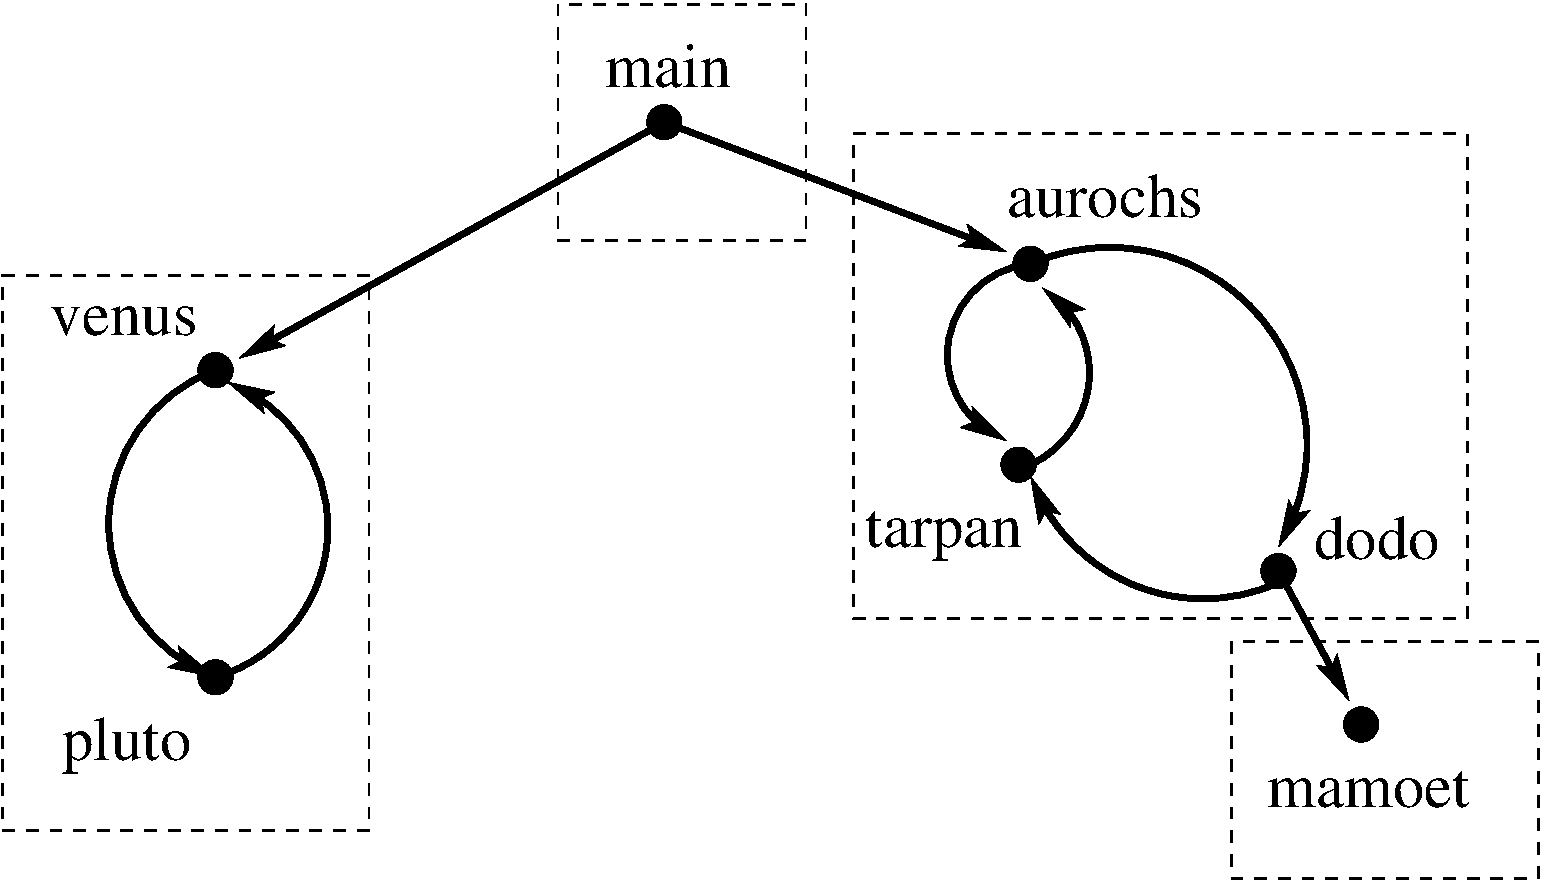
\includegraphics[height=0.2\textheight,keepaspectratio]{vbtarjan}
% \caption{The directed call graph}\label{vbtarjan}
% \end{center}
% \end{figure}
% 
% SCCs partition the program in smaller parts of which the analysis can
% be performed independently, and/or sequentialized
% appropriately. The analysis could concern complexity, invariants (for
% correctness), data-flow, liveness analysis (for optimization) ... One
% finds uses of SCCs in very different contexts.
% 
% 
% The SCCs are indicated in Figure~\ref{vbtarjan} with a rectangle: each
% vertex belongs to exactly one SCC. Try understanding and proving this.
% 
% Algorithm~\ref{alg:tarjan} is an adapted version from
% Wikipedia\footnote{
% http://en.wikipedia.org/wiki/Tarjan's\_strongly\_connected\_components\_algorithm,
% 28-7-2014}.
% %
% Each vertex has 4 fields: the booleans {\em instack} and {\em visited}
% are initially FALSE; the integers {\em index} and {\em lowlink} are
% initialized at a later point in the algorithm. Their selection is denoted as e.g. $v.visited$.
% 
% \begin{algorithm}[h]
% \begin{algorithmic}
% 
% \Function {tarjan}{}
%     \State{index := 1;}
%     \ForAll{$v \in V \wedge (\neg v.visited)$}
%     \State{strongconnect(v);}
%     \EndFor
% \EndFunction
% ~\\
% \Function {strongconnect}{v}
% \State{v.visited := TRUE;}
% \State{v.index := v.lowlink := index++;}
% \State{push(v); v.instack := TRUE;}
% ~\\
% \ForAll {$(v,w) \in E$}
%        \If {$\neg w.visited$};
%        \State{strongconnect(w);}
%        \State{v.lowlink  := min(v.lowlink, w.lowlink);}
%        \ElsIf {w.instack}
%        \State{v.lowlink  := min(v.lowlink, w.index)}
%        \EndIf
% \EndFor
% % ~\\
%     \If{v.lowlink == v.index}
%     \State{start a new SCC}
%     \Repeat
%          \State{w := pop(); w.instack := FALSE;}
%          \State{add w to current SCC}
%     \Until {w == v}
%     \State{output current SCC}
%     \EndIf
% \EndFunction
% 
%   \end{algorithmic}
%   \caption{Tarjan's algorithm computes the SCCs}
%   \label{alg:tarjan}
% \end{algorithm}
% 
% 
% Give arguments why this algorithm ends and is correct.
% 
% Donald E. Knuth\footnote{Turing award in 1974}
% says\footnote{{\bf Twenty Questions for Donald Knuth} at
% \url{http://www.informit.com/articles/article.aspx?p=2213858}} that Tarjan's
% algorithm is his favorite one, also because it sorts topologically as
% a byproduct. Can you see that in the algorithm?




%///////////////////////////////////////////////////////////////////////////////
\chapter{Trees}

%===============================================================================
\section{Introduction}

 \begin{definition}[Tree]
  \textup{ A \textbf{tree} is a simple graph with the property that
there is a unique simple path between any two different points. }
\end{definition}

Any vertex of a tree could be designated as a root of the tree.

 \begin{definition}[Height of a vertex]
  \textup{
The
 \textbf{height of a vertex} $v$ in a tree with root
    $w$, is the number of edges in the path from $w$ to $v$. }
\end{definition}

 \begin{definition}[Height of a tree]
  \textup{
The
\textbf{height of a tree} is the maximum of the heights of its vertices.}
\end{definition}

\begin{figure}[ht]
\begin{center}
\includegraphics[width=0.5\linewidth,keepaspectratio]{bomen1eng}
\end{center}
\caption{Examples of trees \label{bomen1}}
\end{figure}


Figure~\ref{bomen1} shows a tree with root $w$ and a tree without a
root. The heights of $a,b,c,d,e,f,g,h,i$ and $w$ are 1,2,2,1,1,2,3,1,2
and 0.

\begin{figure}[ht]
\centering
\mbox{
\subfigure[ Decision tree]{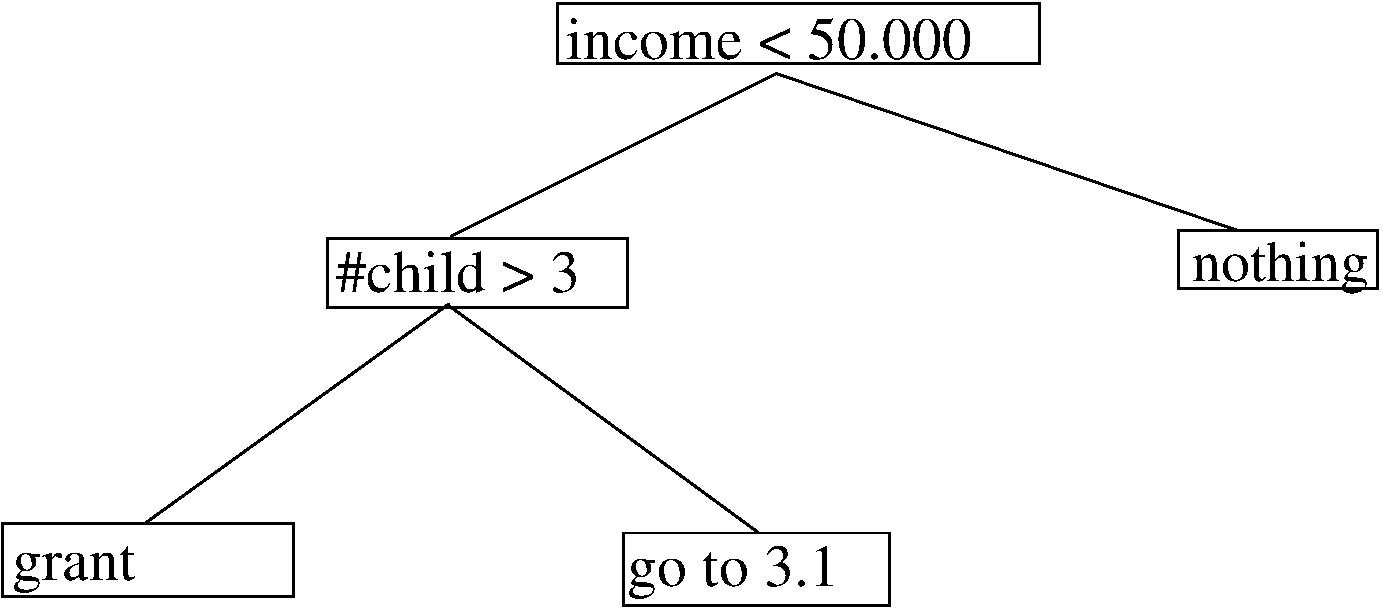
\includegraphics[width=0.5\linewidth,keepaspectratio]{decisiontree1eng} \label{decisiontree1}} %\quad
\subfigure[Representation of $(3+1) *5 - 7/3$]{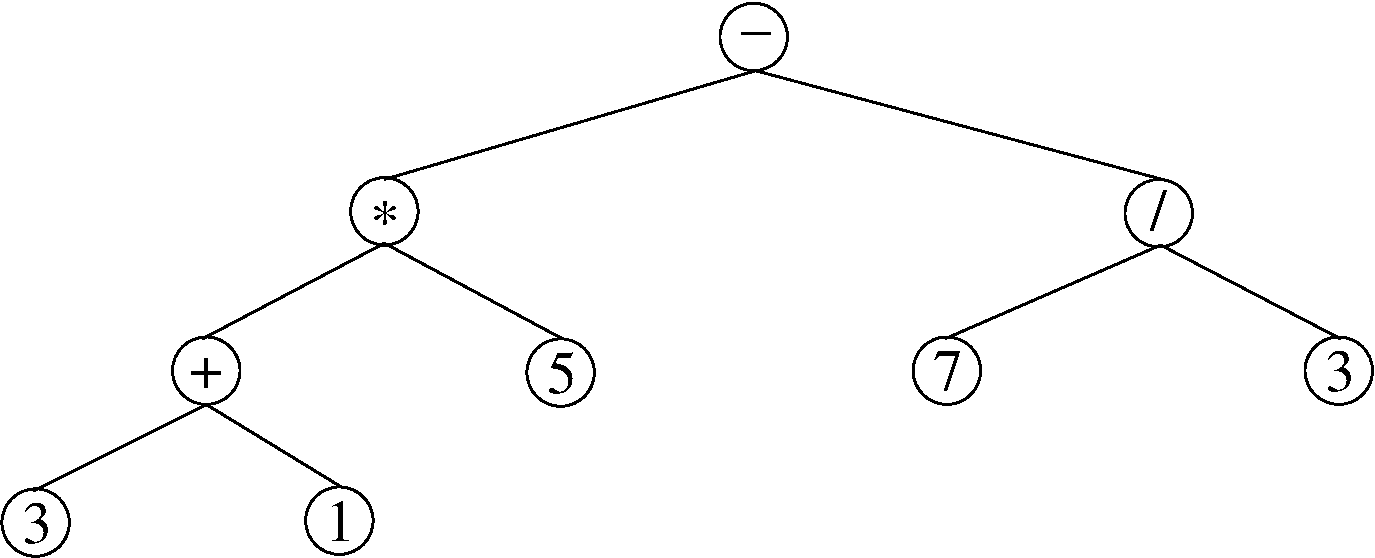
\includegraphics[width=0.5\linewidth,keepaspectratio]{expr1} \label{expr1} }}
\caption{Useful trees}
\end{figure}


Figure~\ref{decisiontree1} shows a decision tree: each vertex
contains a test. The idea is that you start at the root of the tree,
and depending on the answer in the test, you move down left or
right. In this way, you could get advice on whether you are eligible
for financial support.


Figure~\ref{expr1} shows a tree representation of the arithmetic
expression $(3+1) *5 - 7/3$.

%===============================================================================
\section{Properties of Trees}

The following theorem gives 4 equivalent characterisations of trees:

 \begin{theorem}
For a simple graph $T$ with $n$ vertices
 $(a) \Leftrightarrow
  (b) \Leftrightarrow (c) \Leftrightarrow (d)$ with \\[2mm]
(a) $T$ is a tree\\
(b) $T$ is connected and cycle free\\
(c) $T$ is connected and has exactly $(n-1)$ edges\\
(d) $T$ is cycle free and has exactly $(n-1)$ edges
\end{theorem}
\begin{proof} We prove that $(a) \Rightarrow (b)$, $(b) \Rightarrow
(c)$, $(c) \Rightarrow (d)$ and $(d) \Rightarrow (a)$
\begin{itemize}
\item $(a) \Rightarrow (b)$: since $T$ is a tree, there is a path
between any two edges, so $T$ is connected; if $T$ contained a
cycle, some vertices would be connected by more than one path, so $T$
is cycle free
\item $(b) \Rightarrow (c)$:
we prove this by induction on $n$ that $T$ has $(n-1)$ edges; for
$n=1$ $T$ has zero edges, so the basis for the induction is true;
suppose that every connected cycle free graph with $n$ vertices has
$(n-1)$ edges; consider a connected cycle free graph $S$ with $(n+1)$
vertices; choose a simple path $P$ of maximal length in $S$
(convince yourself this is possible); $P$ contains a vertex $v$ with
$\delta(v) = 1$, because there are no cycles in $S$: indeed, when
$\delta(v) > 1$ then one can extend $P$; consider $S \setminus v$ -
the graph $S$ from which $v$ is removed; $S \setminus v$ has $n$
vertices, is cycle free and connected, so by induction $S \setminus v$
has $(n-1)$ edges; consequently, $S$ has $n$ edges

\item $(c) \Rightarrow (d)$: suppose $T$ contains a cycle; we can now
remove at least one edge (and no vertices) from $T$ to obtain a
connected, cycle free graph $T_{*}$; so we can use the previous result
(from $(b) \Rightarrow (c)$), meaning $T_{*}$ has $(n-1)$ edges; this
means that $T$ has strictly more than $(n-1)$ edges, so we get a
contradiction, from which we must conclude that $T$ is cycle free

\item $(d) \Rightarrow (a)$:
we need to prove that $T$ is connected, and that there is a unique
path between every two vertices; consider the partition of $T$ in its
connected components $\{T_{i}\}_{i=1}^{k}$; let the number of vertices
in $T_{i}$ be equal to $n_{i}$; each of the $T_{i}$ is connected and
cycle free, so $T_{i}$ has $(n_{i}-1)$ edges; summing these we get:
$(n-1) = \sum_{i=1}^{k} (n_{i}-1) = \sum_{i=1}^{k} (n_{i}) - k = n - k$;
from this it follows that $k=1$, so $T$ is connected; now suppose that
there exist two different paths from $a$ to $b$: those two paths form
a cycle, but $T$ is cycle free; we conclude that there is a unique
path between every two nodes; so $T$ is a tree

\end{itemize}
\end{proof}

One reason why this theorem is important is this: to walk around in a
general graph is dangerous, because you run the risk to run in circles
(cycles), and your program could easily end up in an infinite loop.
To prevent that, you need to do extra work, for instance keep track of
all the nodes you have visited already. The theorem above tells us
that in a tree, your walk will end if you always go {\em forward},
i.e. never go back to the (one) previous node. The reason is that a
tree has no cycles. So, if you know that you are dealing with trees,
you can and should use that fact in your program.


 \begin{definition}[Terminology related to trees]
\textup{For a tree $T$ with root $v_{0}$, let $x$, $y$ and $z$ be
vertices in $T$ and $(v_{0}, v_{1}, \ldots , v_{n})$ a path.
} {\rm
\begin{verse}
%\begin{itemize}
%\item
\hspace*{1ex}$\bullet$
$v_{n-1}$ is the \textbf{parent} of $v_{n}$; we often say father (or mother)

%\item
\hspace*{1ex}$\bullet$
$v_{0}$ \ldots\ $v_{n-1}$ are all
\textbf{ancestors} of $v_{n}$, and $v_{n}$ is a \textbf{descendant} of
$v_{0}$ \ldots\ $v_{n-1}$
%\item

\hspace*{1ex}$\bullet$
$v_{n}$ is a \textbf{child} of $v_{n-1}$
%\item

\hspace*{1ex}$\bullet$
if $x$ and $y$ have the same parent, then $x$ and $y$ are siblings
%\item

\hspace*{1ex}$\bullet$
if $x$ has no child, $x$ is a \textbf{leaf}, also called {\bf external node}
%\item

\hspace*{1ex}$\bullet$
if $x$ is not a leaf, $x$ is an \textbf{internal node}
%\item

\hspace*{1ex}$\bullet$
a subgraph of $T$ with vertex $x$ and all descendants of $x$, is a
{\bf subtree} of $T$ rooted at $x$\footnotemark
%\end{itemize}
\end{verse}}
\end{definition}
\footnotetext{Actually, you should prove that this subgraph is a tree!}

Relating this to Figure~\ref{boom1}:

\begin{figure}[ht]
\begin{center}
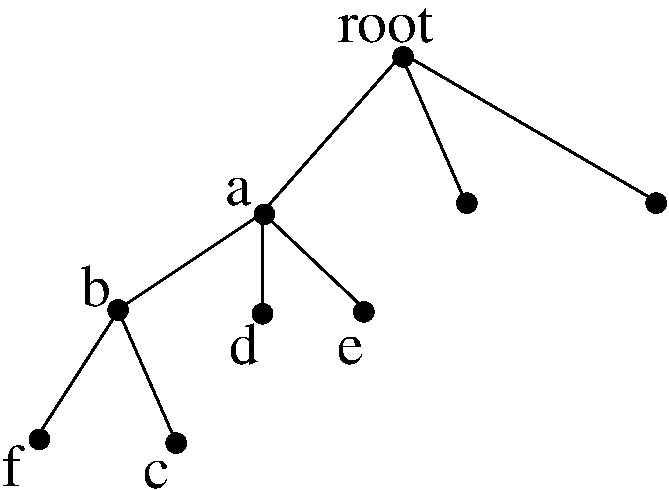
\includegraphics[width=0.25\linewidth,keepaspectratio]{boom1eng}
\end{center}
\caption{Example tree \label{boom1}}
\end{figure}

\begin{itemize}
\item
$c,d,e$ are leaves
\item
$a$ is the parent of $d$
\item
$b,c,f$ are descendants of $a$
\item
$a$ and {\em root} are the ancestors of $b$
\item
$b,d,e$ are siblings
\item
$a,b$ are internal nodes
\item
the subtree rooted in $a$ contains the vertices $a,b,c,d,e,f$
\end{itemize}

Often, the order of the siblings is important, especially with binary
trees.

 \begin{definition}[Binary tree]
\textup{A \textbf{binary tree} is a rooted tree in which every node
has 0, 1, or 2 children; because of the way binary trees are drawn and
used, we speak of a left child (connected to its parent by the left
branch) and a right child (\ldots); this makes an order on the branches
explicit.  }
\end{definition}

You already saw a binary tree in Figure~\ref{decisiontree1}: it is
important to know whether to go left or right on a positive answer to
the test in an internal node.

 \begin{definition}[Full  binary tree]
\textup{A \textbf{full binary tree} is a binary tree
in which every internal node has exactly two children.  }
\end{definition}

\begin{figure}[ht]
\begin{center}
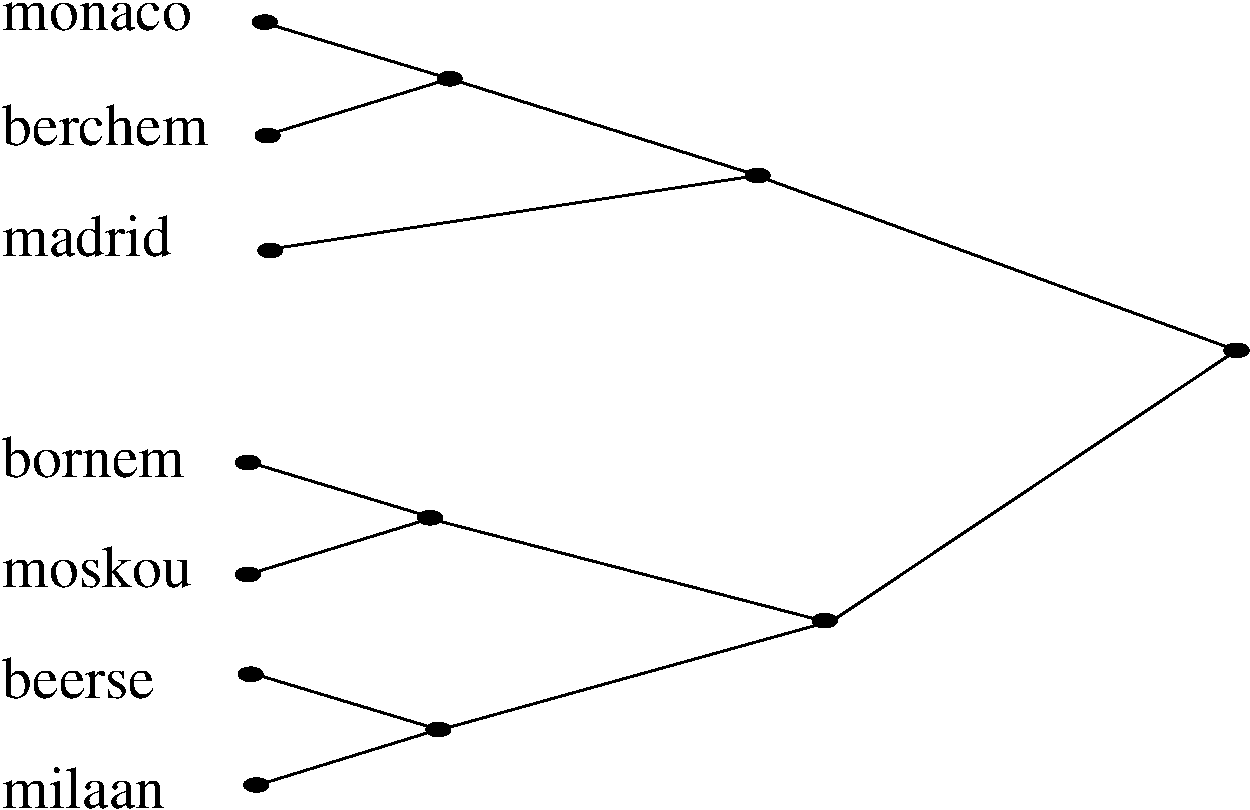
\includegraphics[width=0.5\linewidth,keepaspectratio]{tornooi1}
\end{center}
\caption{Tournament tree \label{tornooi1}}
\end{figure}


Figure~\ref{tornooi1} shows a tournament tree: it is a full binary tree.

 \begin{theorem}
\label{relatiebladinwendig}
A full binary tree $T$ with $i$ internal vertices has
$(i+1)$ leaves and $(2i+1)$ vertices.
\end{theorem}
\begin{proof} Each internal vertex has 2 children, so there are $2i$
children in $T$; there is exactly one vertex that is not a child: the
root; so there are $2i+1$ vertices. Each vertex is either a leaf or
internal, so the number of leaves equals $2i+1 - i = i+1$
\end{proof}


In a tournament with $n$ participants, and direct elimination, you
could wonder how many matches must be played before the winner is
known. Since the tournament tree has $n$ leaves, the number of
internal nodes is $n-1$, and that is the number of matches.

 \begin{theorem}
\label{relatieheightbladeren}
For a binary tree $T$ with height $h$ and $t$ leaves $\log_2(t) \leq
h$ (or $t \leq 2^h$).
\end{theorem}
\begin{proof}
We prove the theorem by induction on $h$ and by considering the
subtrees of $T$: for $h=0$, there is one leaf (the root), so
$t=1=2^h=2^0$ this provides the base case.

Assume $h > 0$; consider $T_{l}$ and $T_{r}$, the left and right
subtree of the root of $T$. $T_{l}$ or $T_{r}$ can be empty, but not both.
Assume $T_{r}$ is empty: then we have $h_{l} = h-1$, and by induction
$t_{l} \leq 2^{h_{l}}$; since $t_{l} = t$ we get $t \leq 2^{h-1}\leq
2^h$.

If $T_{l}$ is empty, we can reason analogously.

Suppose neither $T_{l}$ nor $T_{r}$ is empty; so $h_{l} \leq h-1$ and
by induction $t_{l} \leq 2^{h_{l}}$ and similarly $t_{r} \leq
2^{h_{r}}$, so $t=t_{l} + t_{r} \leq 2^{h_{l}} + 2^{h_{r}}\leq
2^{h-1}+2^{h-1}=2^h$.
\end{proof}

 \begin{theorem} For a binary tree $T$ with $n$ vertices and
height $h$ $\log_2(n+1) \leq h+1$
\label{relatieheightnodes}
\end{theorem}
\begin{proof}
Extend the tree $T$ to a tree $T'$ as follows:
\begin{itemize}
\item
add a left and right branch to every leaf
\item
add a left branch to each internal node missing a left branch
\item
add a right branch to each internal node missing a right branch
\end{itemize}

$T'$ has $n$ internal vertices (all the vertices of $T$) and height
$(h+1)$; $T'$ is full and binary, so we can apply
Theorem~\ref{relatiebladinwendig} and conclude that $T'$ has
$(n+1)$ leaves, and by Theorem~\ref{relatieheightbladeren} $\log_2(n+1)
\leq h+1$.
\end{proof}

Figure~\ref{uitbreiding1} shows a tree and its extension as defined in
Theorem~\ref{relatieheightnodes}: the added vertices are drawn by a
black rectangle. Note that if the original tree is already full, its
extension is different from the original.

\begin{figure}[ht]
\begin{center}
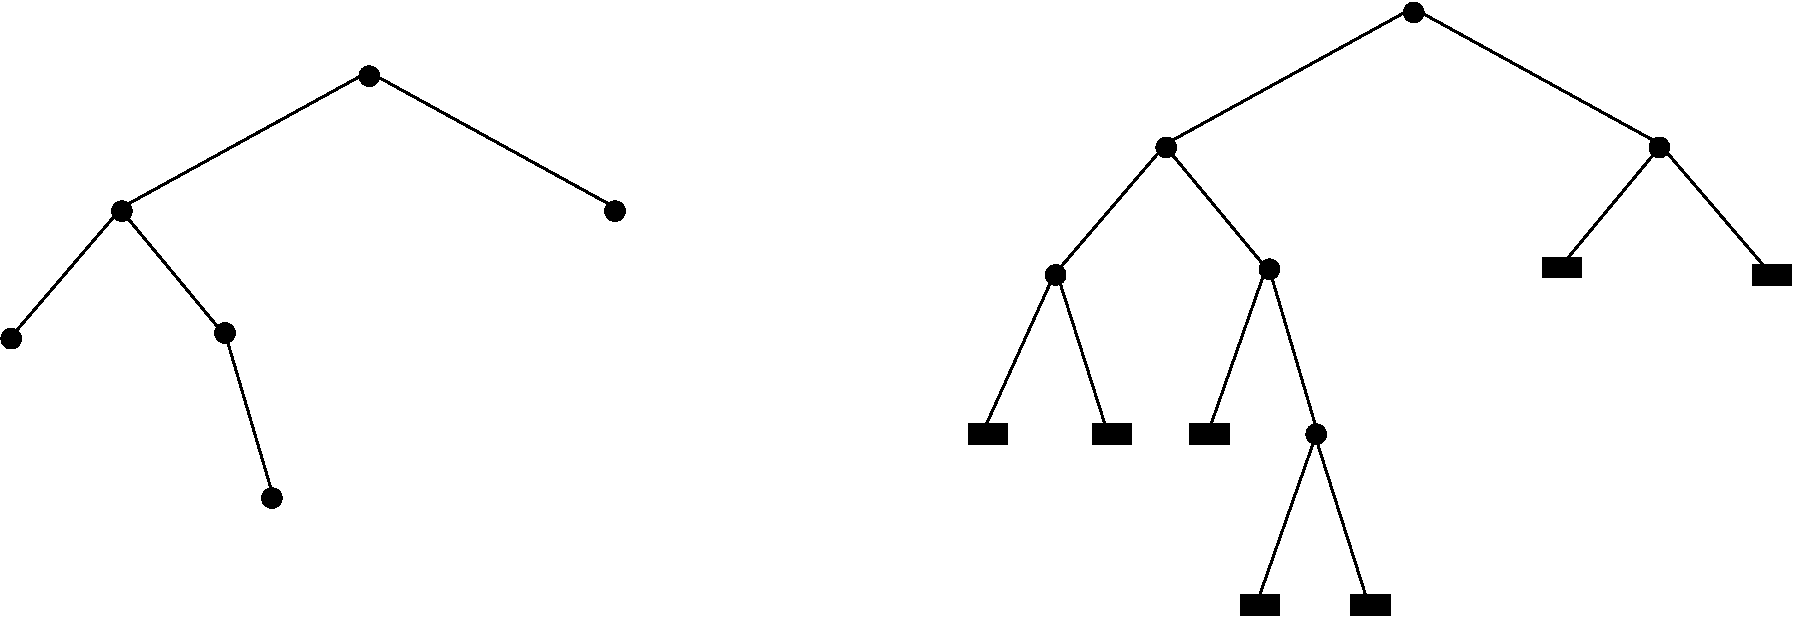
\includegraphics[width=0.6\linewidth,keepaspectratio]{uitbreiding1}
\end{center}
\caption{A binary tree and its extension to a full binary tree\label{uitbreiding1}}
\end{figure}

 \begin{definition}[Binary search tree]
\textup{A \textbf{binary search tree} is a binary tree in which every
vertex $v$ has a value $w(v)$ (e.g. a number or a string) so that
if $l$ belongs to the left subtree of $v$ and $r$ to the right subtree
of $v$, then  $w(l) < w(v) < w(r)$ }
\end{definition}


A binary search tree is also named a sorted binary tree.

Figure~\ref{binboom1} shows a binary search tree in which the values
of the vertices are words; the order is alphabetic.

\begin{figure}[ht]
\begin{center}
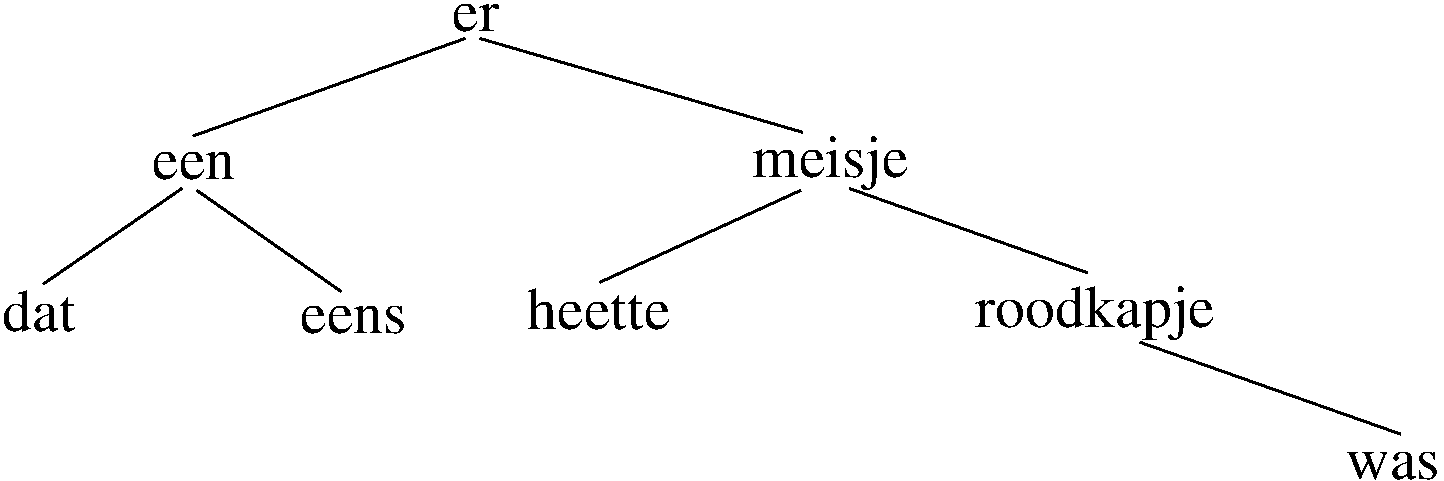
\includegraphics[width=0.6\linewidth,keepaspectratio]{binboom1}
\end{center}
\caption{A binary search tree for the words from the sentence
{\em Er was eens een meisje dat Roodkapje heette} \label{binboom1}}
\end{figure}

The next algorithm searches a given value in a binary search tree: the
algorithm is written as a procedure returning TRUE if the value is
found, and FALSE otherwise.


\parbox{9cm}{
\begin{tabbing}
123456789 \= 12 \= 12 \= 12 \= 12 \= 12 \= 12 \kill
\> boolean search(tree T, value W);\\
\> \{\\
\> \> P = root(T);\\
\> \> while (! empty(P))\\
\> \> \{\\
\> \> \> if (value(P) == W)\\
\> \> \> \> \> return(TRUE);\\
\> \> \> else\\
\> \> \> if (value(P) $<$ W)\\
\> \> \> \> P = rightchild(P);\\
\> \> \> else P = leftchild(P);\\
\> \> \}\\
\> \> return(FALSE);\\
\> \}
\end{tabbing}
}

The complexity of this algorithm can be expressed in the number of
times the body of the while-loop is executed. In the worst case,
the value is not in the tree, and we search along the longest path
starting at the root: that path has length equal to the height $h$ of
the tree, so the loop is executed $h+1$ times. From
Theorem~\ref{relatieheightnodes} we know that $log_2(n+1) \leq h+1$, so
for fixed $n$, the worst case is not less than $log_2(n+1)$. By balancing
the tree as well as possible, we can achieve $\lceil \log_2(n+1)
\rceil$. Figure~\ref{balanced1} shows two binary search trees with the
same values: the one at the right is balanced better than the one on
the left, and has a smaller height.

\begin{figure}[ht]
\begin{center}
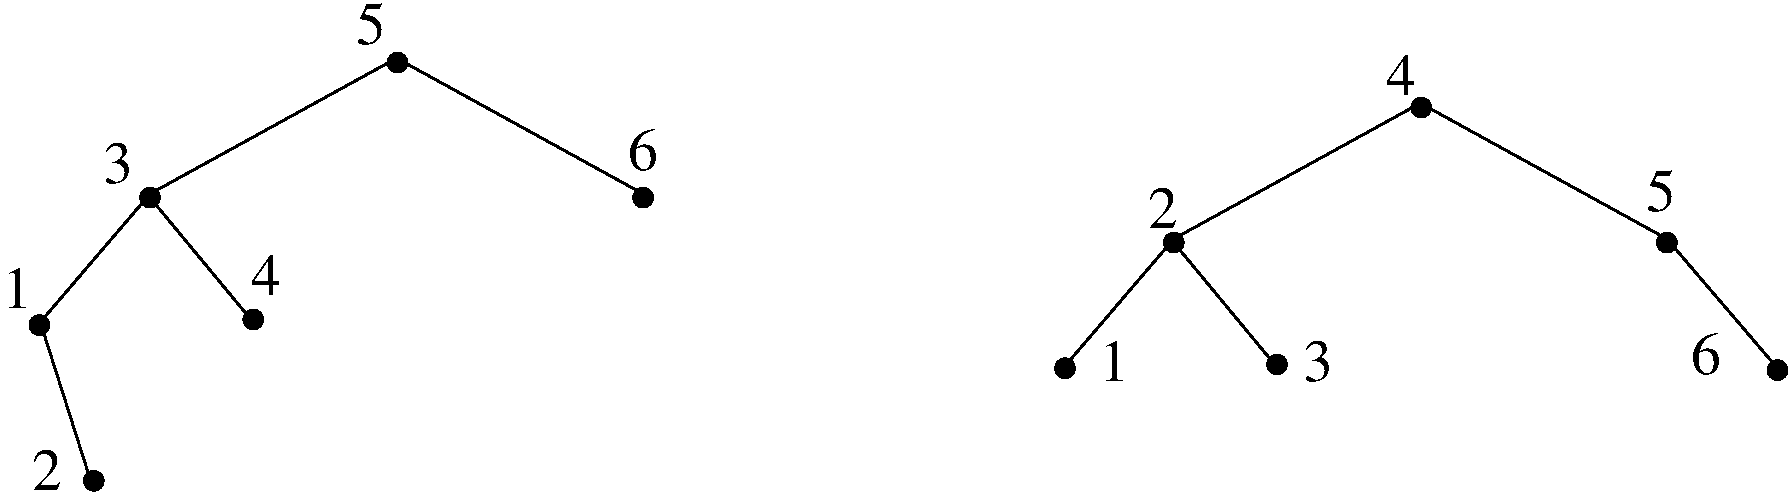
\includegraphics[width=0.6\linewidth,keepaspectratio]{balanced1}
\end{center}
\caption{Two trees with the same values and different height \label{balanced1}}
\end{figure}


%===============================================================================
\section{A Compact Representation}

A tree is often represented with {\em directed} edges. This
representation stresses the fact that often the two functions {\em
leftchild} and {\em rightchild} are explicitly available for use in a
program, but not the function {\em parent}.

It can also be useful to represent a tree as a digraph without cycles
that is not necessarily a tree. As an example take the tree
representation of the expression $(i+7)^{2} + i + 7$ in
Figure~\ref{boomexpressie}. Two subtrees are equal, namely for the
subexpression $i+7$ that occurs twice. The corresponding more compact
representation as digraph can be seen in Figure~\ref{graafexpressie}:
the representation of $i+7$ is now shared.

\begin{figure}[ht]
\mbox{
\hspace{0.5cm}
\subfigure[Tree representation]{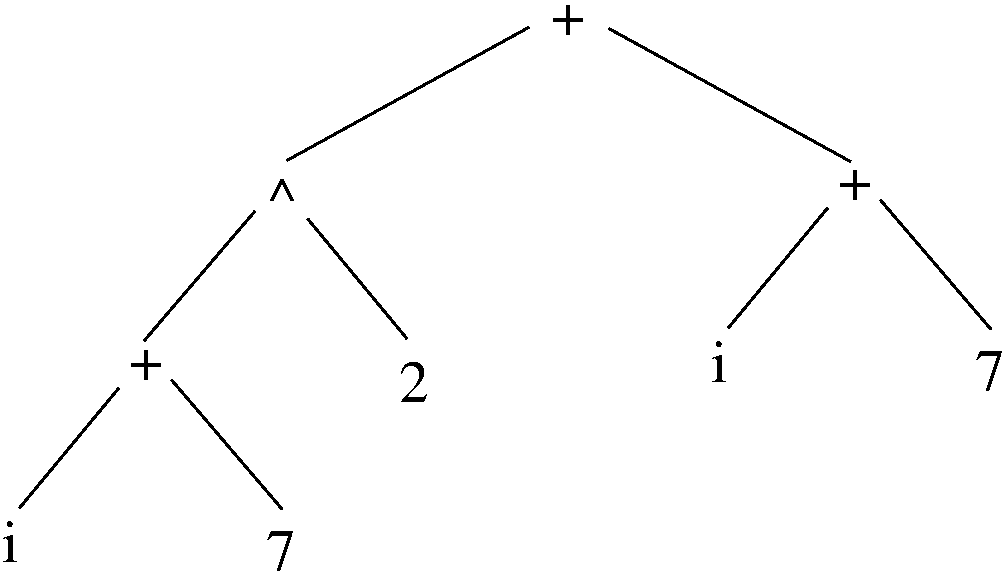
\includegraphics[width=0.4\linewidth,keepaspectratio]{boomexpressie} \label{boomexpressie}}\hspace{1cm}
\subfigure[Graph representation with sharing]{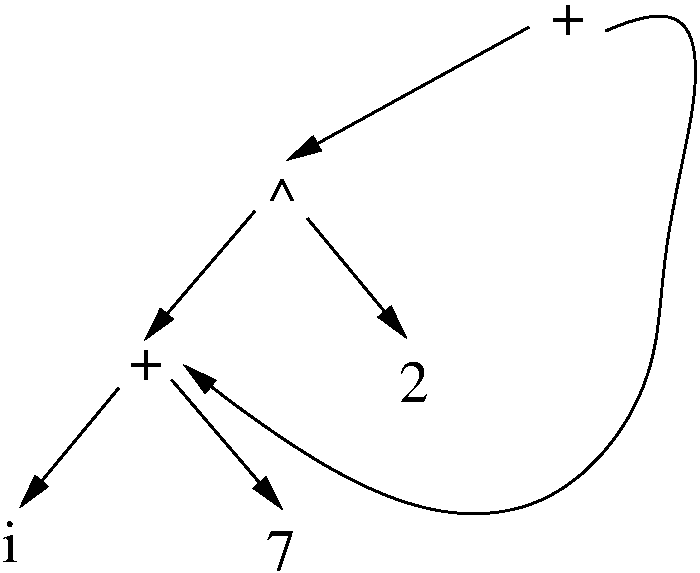
\includegraphics[width=0.3\linewidth,keepaspectratio]{grafeexpressie} \label{graafexpressie} }
}
\caption{Two representations of $(i+7)^{2} + i + 7$}
\end{figure}

Sharing subtrees has its dangers: when the shared subtree is changed,
{\em both} occurrences change. If that is not intended, one should not
use the more compact representation.

%===============================================================================
\section{Spanning Trees}

In this section, we only consider simple graphs: convince yourself
(later) that this is not a severe restriction.

 \begin{definition}[Spanning tree]
A tree \textup{$T$ is a \textbf{spanning tree} of a graph $G$,
if it is a subgraph of $G$ containing all vertices of $G$.}
\end{definition}

A spanning tree covers all vertices of a graph, and it is the smallest
connected subgraph doing so: if you take away an edge from a spanning
tree, you end up with a subgraph that is not a tree.

 \begin{theorem}
A graph $G$ has a spanning tree $T$ if and only if $G$ is connected.
\end{theorem}
\begin{proof}~\\
\begin{itemize}
\item[\fbox{$\Rightarrow$}]
If $G$ has a spanning tree $T$, then $G$ is connected: a path between
any two edges can use the edges of $T$.

\item[\fbox{$\Leftarrow$}]
We prove this direction by induction on the number of cycles $c$ of $G$.
\begin{itemize}
\item[$c = 0$:]
Then $G$ is a tree and a spanning tree of itself.
\item[$c > 0$:]
Remove one edge from a cycle (but not the vertices). The resulting graph $G'$
is still connected and has fewer than $c$ cycles. By the induction hypothesis,
$G'$ has a spanning tree $T$. It should be easy to see that $T$ is also
a spanning tree of $G$.
\end{itemize}
\end{itemize}
\end{proof}

The above theorem does more than prove the existence of a spanning
tree: it gives a constructive method (and algorithm) for finding a
spanning tree: remove an edge from every cycle and you end up with a
spanning tree. An algorithm based on this method is not very
efficient, because we must find cycles and it might be possible to do
better.

\begin{theorem}[Characterisation of spanning tree]\label{opspannend4}
A cycle free subgraph $T$ of a connected graph $G$ that contains a
maximal number of edges of $G$, is a spanning tree of $G$.
\end{theorem}
\begin{proof}

Assume that $G$ has at least 2 vertices.

The fact that $T$ contains a maximal number of edges, means that
that one can't add an edge without introducing a cycle.

We must prove two things: (1) $T$ is connected (which makes it into a
tree); (2) $T$ covers all vertices (making it spanning).


(2) Suppose there exists a vertex $v \in G \backslash T$; since $G$ is
connected, there exits an edge $b$ arriving in $v$; $b \notin T$,
since otherwise $v \in T$; since $T$ is maximal, the graph $T \cup
\{b\}$ contains a cycle that contains $b$. But this means that $v \in
T$, which contradicts the assumption. So $T$ contains all vertices of
$G$.

(1) Suppose that $T$ is not connected; consider the partition of its
components $\{T_{i}\}_{i=1}^{n}$. Figure~\ref{opspannend3} shows
$T_{1}$ and $T_{2}$. Since $G$ itself is connected, there exist
vertices $v_{1} \in T_{1}$ and $v_{2} \in T_{2}$ connected by a simple
path $P$ in $G$ and this path has no other vertices in $T_{1}$ neither
$T_{2}$ (see the dotted line in Figure~\ref{opspannend3}). Suppose $P$
has only one edge $b$. Then $T \cup \{b\}$ contains a cycle through
$v_{1}$ and $v_{2}$; but that means there exists already a path from
$v_{1}$ to $v_{2}$ in $T$, which contradicts the assumption that
$T_{1}$ and $T_{2}$ are two different components.

We still need to prove that in a partition $\{V_{k}\}_{k=1}^{n}$
vertices of a connected graph $G$, there exist always a $V_{i}$ and
$V_{j}$ so that there exist $v_{i} \in V_{i}$, $v_{j} \in V_{j}$, and
an edge $(v_{i},v_{j}) \in G$: consider $V_{1}$ and any other $V_{k}$;
because $G$ is connected, there is a path from a vertex $v_{1} \in
V_{1}$ to a vertex of $V_{k}$; we can choose $v_{1}$ so that the first
edge arrives in a vertex $v \notin V_{1}$. If $v \in V_{k}$, then we
are done. If not, $v$ belongs to another $V_{j}$ and with $j \neq 1$.
\end{proof}


Here is an additional characterisation of spanning trees:

\begin{lemma}
A subgraph of a simple connected graph $G$ with $n$ vertices is a
spanning tree of $G$ if $T$ is cycle free and has $n-1$ edges.
\end{lemma}

\begin{figure}[ht]
\begin{center}
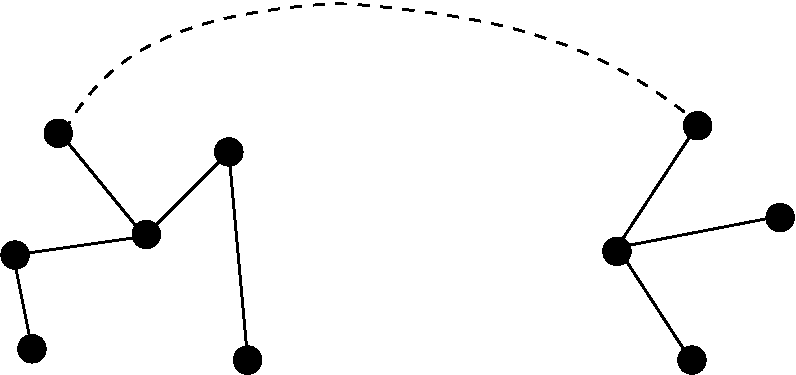
\includegraphics[width=0.3\linewidth,keepaspectratio]{opspannend3}
\end{center}
\caption{Two components of $T$ connected by a path in $G$
\label{opspannend3}}
\end{figure}

Theorem~\ref{opspannend4} leads to a general (non-deterministic)
algorithm for constructing a spanning tree for a graph $G$: start with
the empty tree $T$; repeatedly add an edge to $T$ so that no cycle is
introduced, until this is no longer possible: $T$ is now a spanning
tree.

Note that (1) each edge needs to be considered only once (why?); (2)
the order in which the edges are considered does not matter; (3)
eventually $T$ is a tree, but at intermediate stages, $T$ does not
need to be connected: it is a forest; (4) one can stop trying to add
edges as soon as $T$ has $n-1$ edges.

Two orders for choosing edges are related to general strategies for
tree traversal: {\em depth-first} and {\em breadth-first}. They are
described informally here:

\begin{description}
\item[Depth-first construction of a spanning tree:] choose a vertex
and construct a simple path starting at this vertex with maximal
length: this path belongs to the spanning tree; back up one step along
that path and start at that node constructing a maximal simple path;
repeat backing up and constructing paths ... until you are back at the
initial vertex and can't construct a path anymore;
Figure~\ref{diepteeerst1} illustrates the method starting from the top
vertex: the solid edges belong to the spanning tree.
\begin{figure}[ht]
\begin{center}
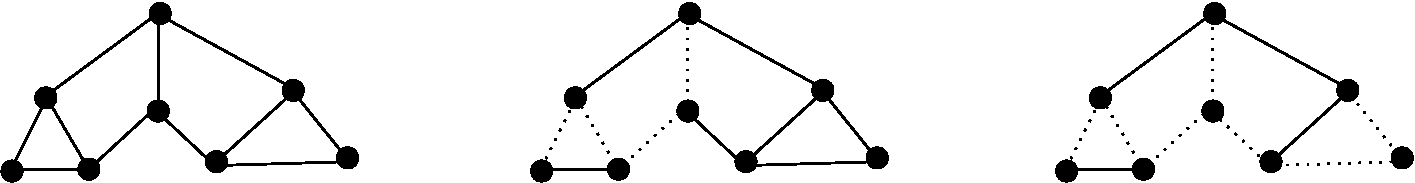
\includegraphics[width=0.6\linewidth,keepaspectratio]{diepteeerst1}
\end{center}
\caption{3 phases in the depth-first construction of a spanning
tree \label{diepteeerst1}}
\end{figure}

\item[Breadth-first construction of a spanning tree:]
choose a vertex and add all edges starting at this vertex while making sure no
cycle is introduced: these edges belong to the spanning tree; repeat this
for all new vertices and keep repeating until no more edge can be
added; Figure~\ref{breedteeerst1} illustrates the method starting from
the top vertex.


\begin{figure}[ht]
\begin{center}
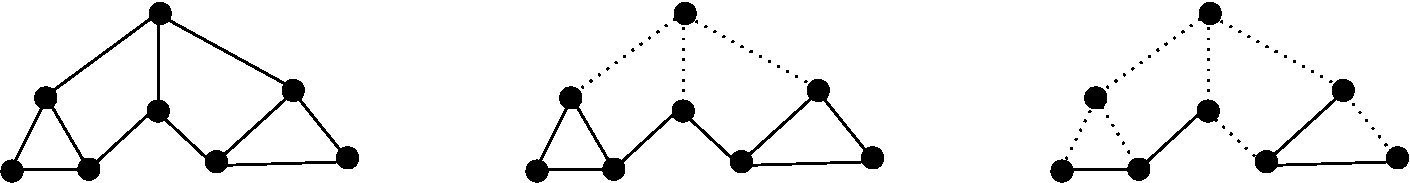
\includegraphics[width=0.6\linewidth,keepaspectratio]{breedteeerst1}
\end{center}
\caption{3 phases in the breadth-first construction of a spanning tree \label{breedteeerst1}}
\end{figure}
\end{description}

The correctness of both methods results from the fact that all edges
are eventually considered for adding to the growing tree, and from
Theorem \ref{opspannend4}. In both methods, the intermediate graph is
a tree, because it is connected and cycle free.

Figure~\ref{opspannend2} shows for $K_{4}$ that depth-first and
breadth-first constructed spanning trees do not need to be isomorphic.

\begin{figure}[ht]
\begin{center}
\includegraphics[width=0.5\linewidth,keepaspectratio]{opspannend2eng}
\end{center}
\caption{Spanning trees for $K_{4}$\label{opspannend2}}
\end{figure}

Maybe you think that {\bf all} spanning trees can be obtained by
either method, but Figure~\ref{opspannend5} shows a graph with a
spanning tree that neither of the methods can compute.

\begin{figure}[ht]
\begin{center}
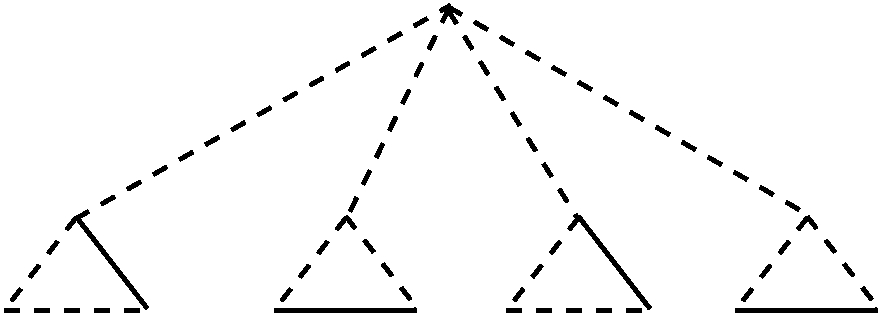
\includegraphics[width=0.5\linewidth,keepaspectratio]{opspannend5}
\end{center}
\caption{Graph with a hybrid spanning tree\label{opspannend5}}
\end{figure}

%===============================================================================
\section{Minimal Spanning Trees}

Consider the following problem: there are a number of cities between
which a road network must be built. The cost of building any road
between two cities is known (it is always strictly positive). We want
to choose which cities to connect by a road, while satisfying two
criteria: (1) the total cost must be minimal, (2) each city must be
reachable from any other city.

Clearly, the network has to be a tree because it can't have cycles
(otherwise the cost would not be minimal), and it must be connected.
This kind of trees is defined as:

 \begin{definition}[Minimal spanning tree (MST)]
\textup{$T$ is a \textbf{minimal spanning tree} of a weighted graph
$G$ if $T$ is a spanning tree of $G$ with minimal weight.}
\end{definition}

Figure~\ref{opspannend1} shows a graph, one of its spanning trees, and
its minimal spanning tree.

\begin{figure}[ht]
\begin{center}
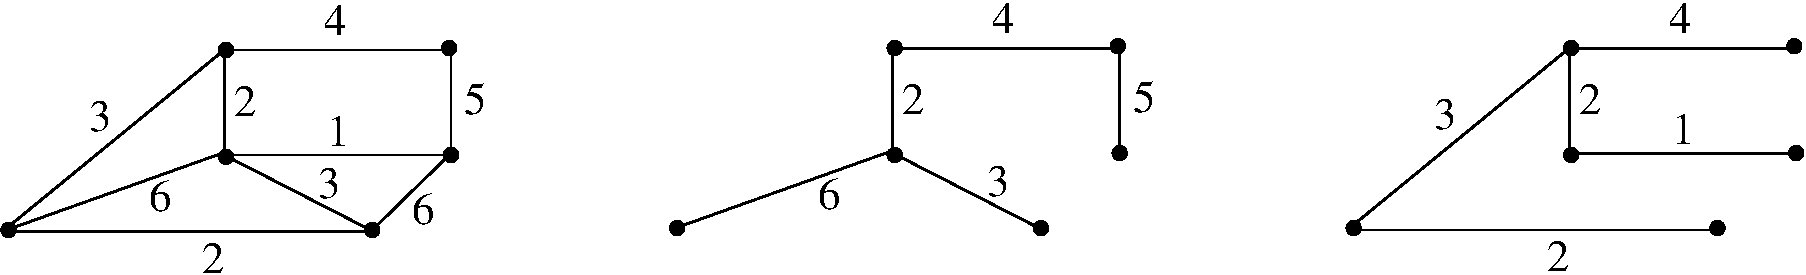
\includegraphics[width=0.6\linewidth,keepaspectratio]{opspannend1}
\end{center}
\caption{A graph with spanning trees\label{opspannend1}}
\end{figure}

Can a graph have more than one MST? Does a graph always have at least
one MST?

Efficient algorithms for constructing an MST are based on the following
theorem:

\begin{theorem} An edge that belongs to an MST \label{even}

Let $(V,E)$ be a connected graph, $U \subset V$ and $e \in E$
so that $e$ has minimal length of all edges between $U$ and $V
\backslash U$. Then $e$ belongs to some minimal spanning tree $T$ of
$(V,E)$.
\end{theorem} % stelling 2.3 from Shimon Even
\begin{proof} Let $T_{0}$ be any MST of $(V,E)$. If $e \in T_{0}$,
then we are done. If not, add $e$ to $T_{0}$, resulting in $T_{1}$
which contains a cycle (Theorem~\ref{opspannend4}). This cycle
contains $e$ and also another edge $e' = (u,v)$ so that $u \in U$ and
$v \in V \backslash U$. Removing $e'$ from $T_{1}$ results in a
spanning tree $T$ (why is $T$ a tree?) and moreover $w(T) \leq
w(T_{0})$ since $w(e) \leq w(e')$. So, $T$ is a minimal spanning tree
containing $e$.
\end{proof}


\begin{code}Prim\label{prim} \\
  Let $G(V,E)$ be a connected weighted graph where the
vertices are numbered: $V = \{v_{1},v_{2},\ldots,v_{n}\}$. The
following procedure constructs a minimal spanning tree $T$ for $G$.
\begin{enumerate}
\item \textbf{Initialisation}: $T := (\{v_{1}\},\emptyset)$
\item \textbf{Stop?}: If $T$ has $(n-1)$ edges, stop.
\item \textbf{Add edge}:
Define $S = \{e | e = (u,v), u \in T, v \notin T\}$ and choose an edge
$b$ from $S$ so that $\forall e \in S: w(b) \leq w(e)$. Add $b$ to
$T$. The result is still connected and cycle free.
Go to \textbf{Stop?}.
\end{enumerate}
\end{code}

\begin{proof}
At the end of the algorithm, $T$ is a tree with $n$ vertices,
$(n-1)$ edges, and cycle free, so $T$ is a spanning tree $G$. We still need to prove termination of the algorithm and the minimality of $T$.

Termination is easy: \textbf{Add edge} is executed $(n-1)$ times, and
then the algorithm stops. Maybe you should convince yourself that
\textbf{Add edge} is always possible as long as $T$ has less than
$n-1$ edges.

Figure \ref{prim2} shows the reasoning below.

After the \textbf{Initialisation}, $T$ consists of one vertex, so at
that moment $T$ is part of an MST. We now prove that this property
is invariant under the application of \textbf{Add edge}:

denote by $W$ the vertices of $T$ and suppose that $T \subset T'$ with
$T'$ an MST. Denote by $B$ the set
%
$\{(x,y)\;|\; x \in W,\; y \in V \backslash W,\; (x,y) \in E\}$.
%
Consider a shortest edge $(i,j)$ in $B$ that does not cause a cycle
when added to $T$. If $(i,j) \in T'$ then clearly $T \cup \{(i,j)\}
\subseteq T' = $ MST. If $(i,j) \notin T'$ then $T' \cup \{(i,j)\}$
contains a cycle which contains $(i,j)$.  This cycle contains another
edge $(x,y) \in B$ and we can take it out of $T' \cup \{(i,j)\}$ so
that we get a new spanning tree $T''$ (it contains all vertices and is
connected and cycle free). So the question is: is $T''$ minimal?
Since $w(i,j) \leq w(x,y)$ (that is how $(i,j)$ was chosen), we
have $w(T'') \leq w(T')$ so $T''$ is an MST. We can conclude that
$T \cup \{(i,j)\}$ is part of an MST.

As a result, the spanning tree constructed by Prim is a minimal
spanning tree.
\end{proof}

\begin{figure}[ht]
\begin{center}
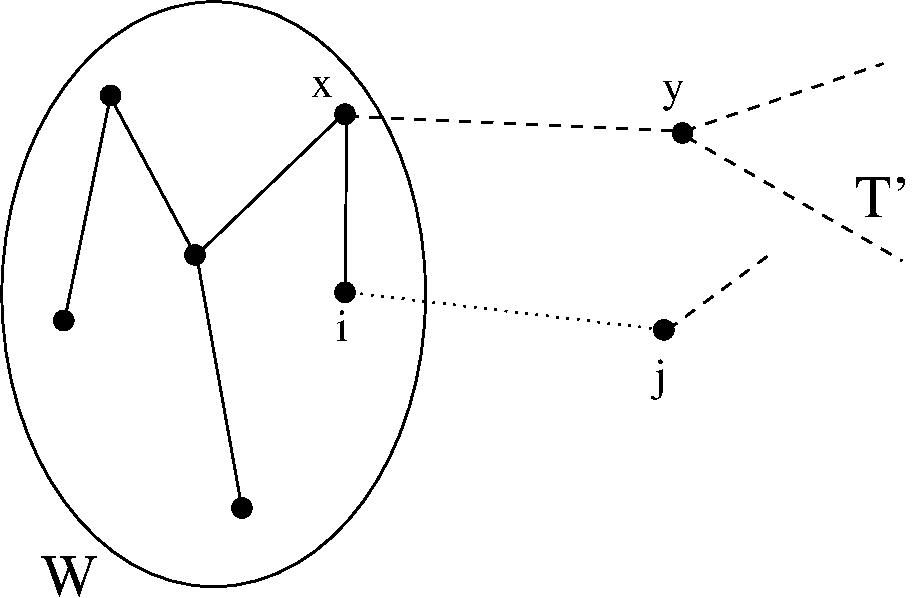
\includegraphics[width=0.4\linewidth,keepaspectratio]{prim2}
\end{center}
\caption{Illustration of the Algorithm~\ref{prim} \label{prim2}}
\end{figure}


Prim's algorithm is a classic example of a {\em greedy} algorithm: any
time a choice needs to be made, the decision is made taking very
little into account, and definitely not the future choices. Exactly
because of Theorem \ref{even}, this greedy algorithm delivers the
optimal solution. That is not true for every greedy algorithm: a
shortest path algorithm that would choose at any junction the shortest
edge leaving that junction, often does not give an overall shortest
path; also, a greedy chess player loses more often than they win.

Prim's algorithm is illustrated in Figure~\ref{prim1}: the initial
vertex is A; the order in which the edges are added, is indicated as
a,b,c \ldots h.

\begin{figure}[ht]
\begin{center}
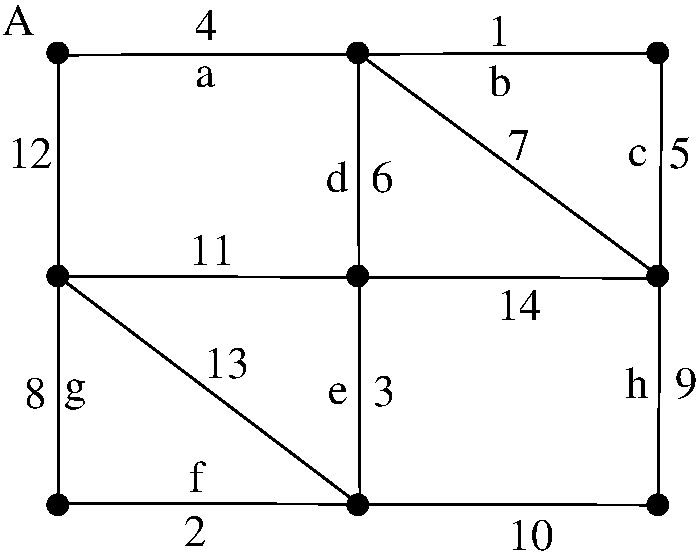
\includegraphics[width=0.3\linewidth,keepaspectratio]{prim1} % ,height=5cm}
\end{center}
\caption{Prim's algorithm~(\ref{prim}) executed \label{prim1}}
\end{figure}


Prim's algorithm builds the MST incrementally: at each moment during
the execution of the algorithm, $T$ is an MST of a subgraph of
$G$. There is also a variant of Prim's algorithm without this
property:


\begin{code} Kruskal \label{kruskal}\\
  Let $G(V,E)$ be a connected weighted graph $G(V,E)$ where the
vertices are numbered: $V = \{v_{1},v_{2},\ldots,v_{n}\}$. The
following procedure constructs a minimal spanning tree $T$ for $G$.
\begin{enumerate}
\item \textbf{Initialisation}: $T := \emptyset$
\item \textbf{Stop?}: If $T$ has $(n-1)$ edges, stop.
\item \textbf{Add edge}: Add to $T$ an edge $b$ with minimal weight
  that does not introduce a cycle in the result. Go to {\bf Stop?}.
\end{enumerate}
\end{code}
\begin{proof}
Termination of Kruskal is proven as for Prim.

The proof that $T$ is a spanning tree at the end, is also similar.

We prove minimality of $T$. Assume $T$ is not an MST.  Name the edges
of $T$ $b_{1},b_{2},\ldots ,b_{n-1}$ in the order as added by the
algorithm. Let $S$ be an MST of $G$ so that
%
$\{b_{1}, b_{2}, \ldots , b_{i}\} \subseteq S$ and with maximal $i$
(such an $S$ exists and by Theorem~\ref{even} $i \geq 1$!). There are
now two possibilities:
\begin{itemize}
\item
\textbf{$i = n-1$}: this means that $T = S$ so $T$ is an MST.
\item
\textbf{$i < n-1$}: now $b_{i+1} \notin S$; let $H$ be the graph with
the edges $\{b_{1}, b_{2}, \ldots , b_{i}\}$ (and their
vertices). Consider the graph $S \cup \{b_{i+1}\} = S'$. $S'$ has a
cycle with at least one edge $b$ not belonging to $T$ (because $T$ is
itself cycle free). So, $b \in S$. $H \cup \{b\}$ is cycle free,
because $H \cup \{b\} \subseteq S$ and since Kruskal added edge
$b_{i+1}$ in the $(i+1)^{th}$ \textbf{Add edge} (for addition to $H$),
we know that $w(b_{i+1}) \leq w(b)$. Consequently $S' \backslash \{b\}
= S''$ is an MST. But that makes $S''$ into an MST that contains
$\{b_{1}, b_{2}, \ldots , b_{i+1}\}$, in contradiction with the
maximality of $S$. It follows that $i < n-1$ is not possible.
\end{itemize}
\end{proof}

Note that during Kruskal, $T$ does not need to be a tree all the
time. The execution of Kruskal's algorithm is illustrated in
Figure~\ref{kruskal1} on the same graph as in Figure~\ref{prim1}.

\begin{figure}[ht]
\begin{center}
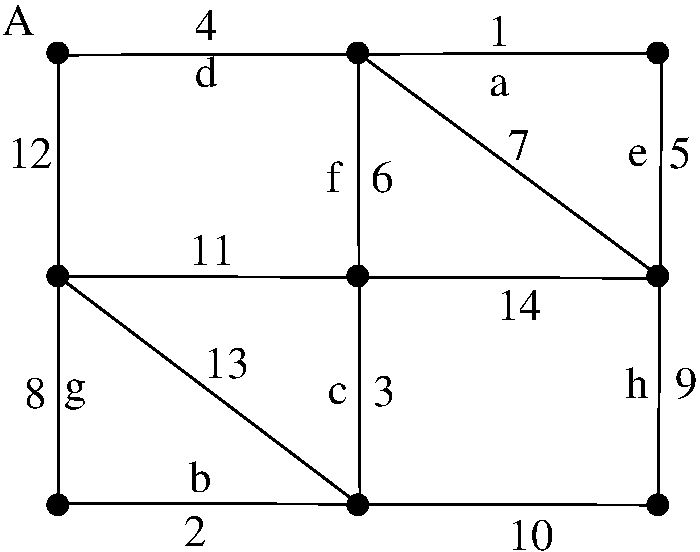
\includegraphics[width=0.3\linewidth,keepaspectratio]{kruskal1} % ,height=5cm}
\end{center}
\caption{Kruskal's algorithm executed}\label{kruskal1}
\end{figure}


%///////////////////////////////////////////////////////////////////////////////
\chapter{Network Models}

A network of connections with each having its own capacity can be modelled by
a directed, weighted graph. The following are examples of such
networks: a road network, an electrical network, oil pipes \ldots An
interesting and important problem in this area is the optimization
of the flow, while respecting the capacities. We will solve this
optimization problem with some graph theory. Problems that are
seemingly unrelated to flow optimization can often be modelled as a
network problem as well: personnel assignment, resource allocation and
even partner choice - the latter is known as the {\em marriage
  problem}.


%===============================================================================
\section{Transport Networks}

 \begin{definition}[Transport network] {\rm A \textbf{transport
         network} (or simply \textbf{network}) is a simple, weighted,
       directed graph $G$ with the following properties:
\begin{verse}
1. there is exactly one vertex in $G$ without incoming edges; this
vertex is called the \textbf{source}

2. there is exactly one vertex in $G$ without outgoing edges; this
vertex is called the \textbf{sink}

3.
the weight $C_{i,j}$ of the (directed) edge $(i,j)$ is positive and is
named the \textbf{capacity} of the edge

4.
disregarding the direction of the edges, $G$ is connected
\end{verse}
}
\end{definition}



Figure~\ref{transport1} shows a network: the source is vertex $a$ and
the sink is $z$; the capacity of an edge is written next to the
edge. The network could model a number of one way streets in a city
with a railway station $a$ and a market place $z$; the capacity could
be the number of vehicles that can pass through the street per minute.

\begin{figure}[ht]
\begin{center}
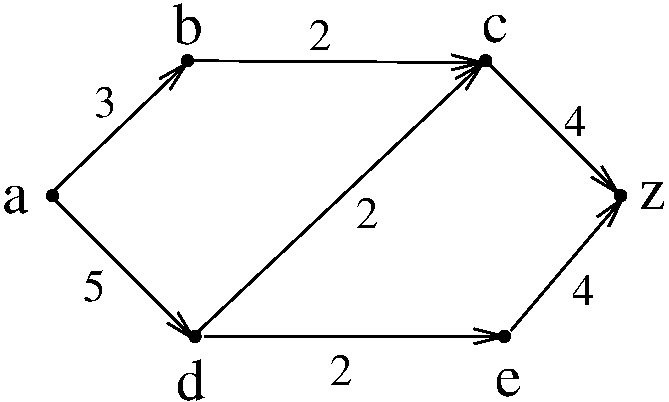
\includegraphics[width=0.3\linewidth,keepaspectratio]{transport1} % ,height=3cm}
\end{center}
\caption{A transport network \label{transport1}}
\end{figure}

The restriction to simple graphs is not so bad: loops and parallel
edges can be simply removed by putting an extra vertex on such
edges. This changes nothing essential as far as the problems studied
later in this section are concerned.


\begin{definition}[Network flow]\label{stroming1}
\label{stromingdef}
{\rm A {\bf network flow} $F$ in a network $G(V,E)$ with capacities
  $C_{i,j},\;\; i,j \in V$\footnotemark is a mapping from $E$ to
  $\R^{+}$ so that\\
\begin{minipage}{12cm}
\begin{enumerate}
\item
\label{stromingdef1}
$F(i,j) \leq C_{i,j}$
\item \label{conserve1} for each vertex $j$ different from source and
  sink:
\[\displaystyle \sum_{i \in V} F(i,j) = \sum_{i \in V} F(j,i)\]
\end{enumerate}
\end{minipage}\\[2mm]
We name $F(i,j)$ the flow in edge $(i,j)$. For a vertex $j$, we name
the quantity $\sum_{i \in V} F(i,j)$ the incoming flow in $j$, and
$\sum_{i \in V} F(j,i)$ the outgoing flow out of $j$.  }
\end{definition}
\footnotetext{if there is no edge $(i,j)$, we assume that $C_{i,j} = 0$}



Formula~\ref{conserve1} in Definition~\ref{stroming1} expresses the
law of conservation of goods: everything that comes into an edge must
get out as well. That prevents accumulation of goods in a vertex, and
production of goods in a vertex. Think of Kirchhoff's law.

Figure~\ref{stroom2} shows a flow for the network of Figure
\ref{transport1}; the flow is defined by:
\begin{center}
$
\begin{array}{l}
F(a,b) = 2\\
F(b,c) = 2\\
F(c,z) = 3\\
F(a,d) = 3\\
F(d,c) = 1\\
F(d,e) = 2\\
F(e,z) = 2\\
\end{array}
$
\end{center}
It is marked next to the capacity of the corresponding edge.
\begin{figure}[ht]
\begin{center}
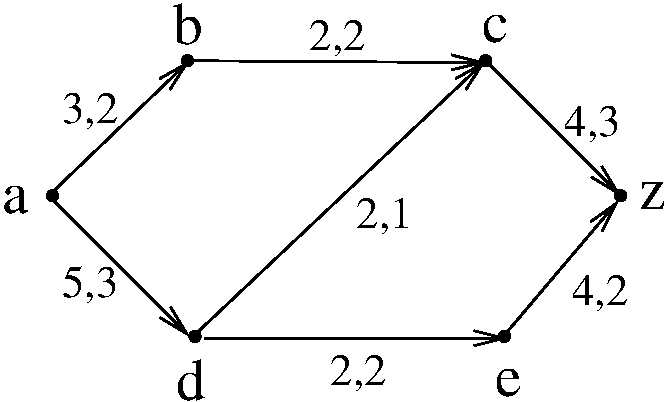
\includegraphics[width=0.3\linewidth,keepaspectratio]{stroom2} % ,height=3cm}
\end{center}
\caption{A transport network flow \label{stroom2}}
\end{figure}

You can check that Formula~\ref{conserve1} in
Definition~\ref{stroming1} is satisfied for each vertex, except the
source and the sink.

You can also check that the flow coming out of the source equals the
flow coming into the sink.

\begin{center}
\mbox{$F(a,b)+F(a,d) = F(c,z) + F(e,z)$}.
\end{center}
This equality is more generally true:

 \begin{theorem}[Source-out = sink-in] \label{source=sink}
For any flow $F$ in a network $G(V,E)$, the flow coming out of the
source equals the flow going into the sink, or more formally:
\[\sum_{i \in V} F(a,i) = \sum_{i \in V} F(i,z).\]
\end{theorem}
\begin{proof}

It should be clear that

$~~~~~~~~~~\sum_{j \in V} (\sum_{i \in V} F(i,j))  =
                \sum_{i \in V} (\sum_{j \in V} F(i,j))
         =  \sum_{j \in V} (\sum_{i \in V} F(j,i))$

Interchanging the $\sum$'s is allowed as we are dealing with finite
graphs. The second equality holds because we only renamed $i$ and $j$.

It follows that

\begin{tabular}{c c c l}
~~~~~~~~~ &
0 & = & $\sum_{j \in V} \left(\sum_{i \in V} F(i,j) - \sum_{i \in V} F(j,i) \right)$\\
 & & & \\
 &  & = & $\left( \sum_{i \in V} F(i,z) -  \sum_{i \in V} F(z,i)\right) +
                \left(\sum_{i \in V} F(i,a) -  \sum_{i \in V} F(a,i)\right)$
    \\
 & & & \\
 &  &  & \hspace*{2cm}
       $+ \sum_{j \in V \backslash \{a,z\}} \left( \sum_{i \in V} F(i,j) -
                \sum_{i \in V} F(j,i)\right)$\\
 & & & \\
 & & = & $\sum_{i \in V} F(i,z) - \sum_{i \in V} F(a,i)$
\end{tabular}



since $F(z,i) = 0 = F(i,a)$ for $\forall i \in V$ (by Definition~\ref{stromingdef})

and  $\sum_{i \in V} F(i,j) = \sum_{i \in V} F(j,i)$  $\forall j \in
(V \backslash \{a,z\})$ (by Formula~\ref{conserve1} in
Definition~\ref{stromingdef})
\end{proof}



Theorem~\ref{source=sink} justifies the following:

 \begin{definition}[Value of a flow]
\textup{The \textbf{value of a flow $F$} in a network $G(V,E)$
with source $a$ and sink $z$ is $\sum_{i \in V} F(a,i)$ or
$\sum_{i \in V} F(i,z)$ }
\end{definition}

The value of the flow in Figure~\ref{stroom2} is 5.



The network problem can now be formulated as: for a given network $G$,
find a maximal flow, i.e. a flow with maximal value.


Before we go into that \ldots Networks could have more than one source
and/or sink: the network in Figure~\ref{transport2} could represent
the water supply of cities $A$ and $B$, from sources $X,Y$ and $Z$,
and with intermediate distribution centers $b,c$ and $d$.

\begin{figure}[ht]
\begin{center}
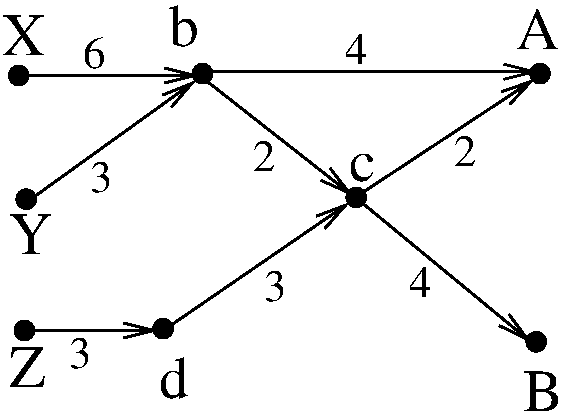
\includegraphics[width=0.22\linewidth,keepaspectratio]{transport2} % ,height=3cm}
\end{center}
\caption{A transport network with more than one source and sink \label{transport2}}
\end{figure}

One can add a super source $a$ and a super sink $z$ to the network, an
edge from $a$ to each original source with infinite capacity, and an
edge from each sink to the super sink, also with infinite capacity: we
get the usual network.

\begin{figure}[ht]
\begin{center}
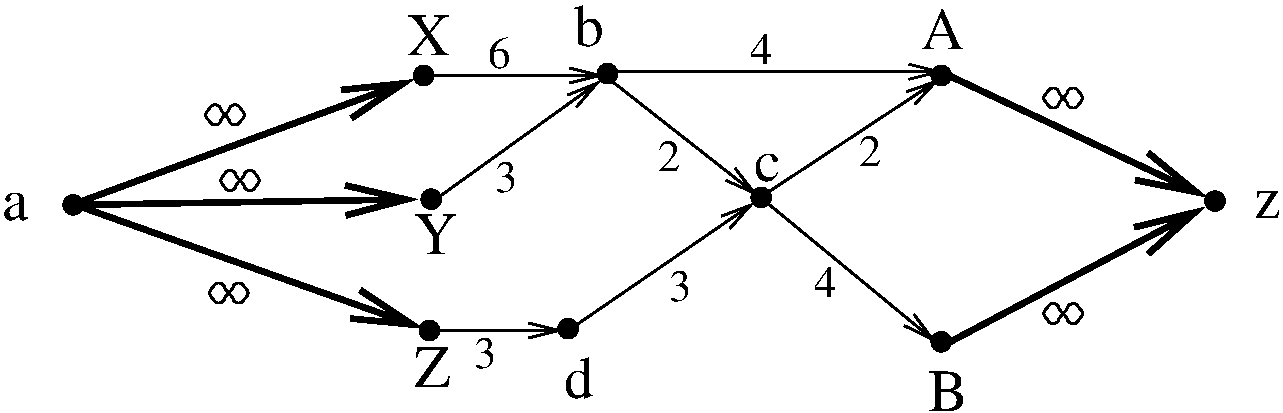
\includegraphics[width=0.507\linewidth,keepaspectratio]{transport3} % ,height=3cm}
\end{center}
\caption{The same transport network with a super source and a
super sink \label{transport3}}
\end{figure}

A maximal flow in the new network corresponds to a maximal flow in the
original network: convince yourself of that.

Finally, a maximal flow is often not unique: Figure~\ref{stroom3}
shows a network with infinitely many maximal flows. Indeed, for each
$i$ and $j$ satisfying $i+j = 5$ and $0 \leq i,j \leq 3$, the flow is
maximal.

\begin{figure}[ht]
\begin{center}
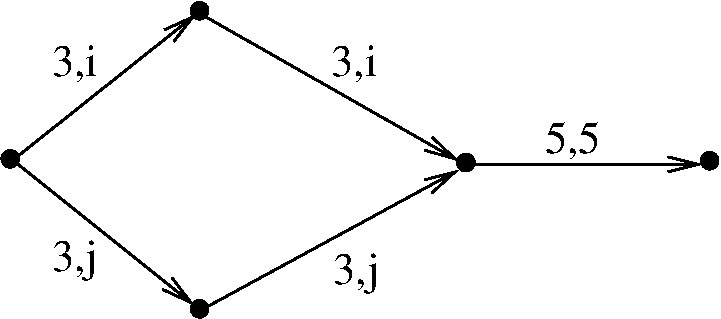
\includegraphics[width=0.3\linewidth,keepaspectratio]{stroom3} % ,height=2.5cm}
\end{center}
\caption{A network with infinitely many maximal flows\label{stroom3}}
\end{figure}


%===============================================================================
\section{Maximal Flow}

The idea behind the next algorithm for computing a maximal flow is as
follows: start from any flow and improve it until no longer possible -
you end up with a maximal flow. The informal description of how to
improve a flow is:
\begin{itemize}
\item
consider a path $P$ from the source $a$ to the sink $z$
\item
find the minimum $\Delta$ of $C_{b} - F(b)$ over all edges $b \in P$
\item
construct the new flow along path $P$ by adding $\Delta$ to each $F(b)$
\end{itemize}

A few remarks about this recipe:
\begin{itemize}
\item the operation increases the flow if and only if $\Delta > 0$
along that chosen path $P$
\item the above only works if all edges in $P$ have the correct (the
{\em good}) direction, but
\item limiting ourselves to paths from $a$ to $z$ along the directed
edges is not enough: look at Figure~\ref{transport4}; no path with
only good edges can be improved with the above method; but the flow
along the path $(a,b,c,z)$ can be improved: the resulting flow is
shown in Figure~\ref{transport5};

\begin{figure}[ht]
\begin{center}
\subfigure[A non-maximal flow]{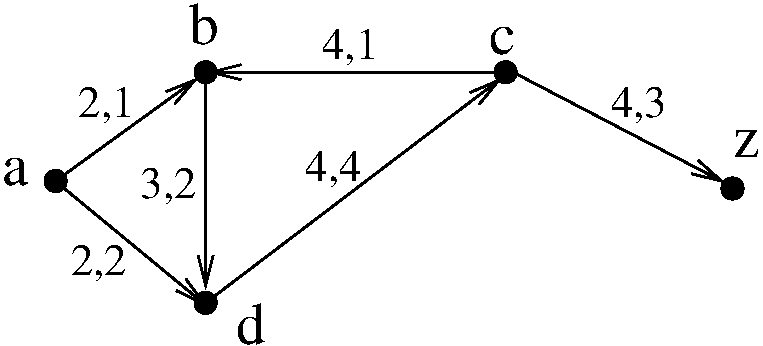
\includegraphics[width=0.3\linewidth,keepaspectratio]{transport4} \label{transport4}}\hspace{1.2cm}
\subfigure[A better flow along a path with a {\em bad}
edge]{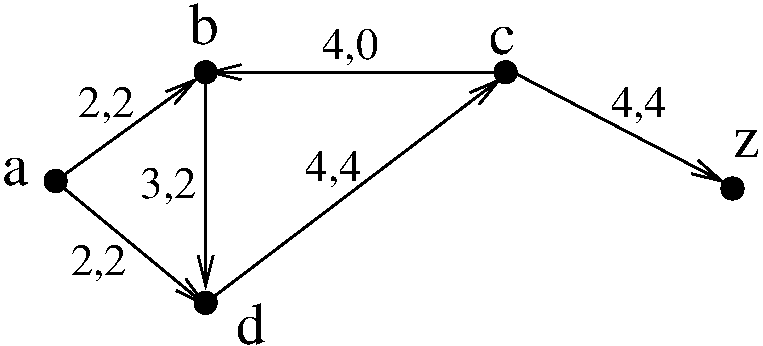
\includegraphics[width=0.3\linewidth,keepaspectratio]{transport5} \label{transport5}}
\end{center}
\caption{Improving a flow}
\end{figure}

It follows that we also need to consider paths with inverted edges,
and we don't add a $\Delta$ to them, we subtract it: if an inverted
edge has a non-zero flow, it is possible that some flow is running in
cycles without ever reaching the sink, while still using up the
capacity of some edges. We formalize this now.

\end{itemize}

 \begin{definition}[Good and bad edges]
\textup{In a digraph $G(V,E)$ with path $(v_{1},v_{2},\ldots ,v_{n})$
we name an edge $(v_{i},v_{i+1})$ \textbf{good} if $(v_{i},v_{i+1})
\in E$, and otherwise \textbf{bad}}
\end{definition}

In a path $P$, we denote the good edges by $P_{+}$, the bad edges by $P_{-}$.


 \begin{theorem} Improving a flow
\label{verbeterflow}\\
Let $P$ be a path from $a$ to $z$ in a network $G(V,E)$, so that
\begin{verse}
1.
$\forall (i,j) \in P_{+}$: $F(i,j) < C_{i,j}$

2.
$\forall (i,j) \in P_{-}$: $0 < F(i,j)$
\end{verse}

Define $\Delta$ as $min(min_{(i,j) \in P_{+}}
\{C_{i,j}-F(i,j)\},min_{(i,j) \in P_{-}} \{F(i,j)\})$, and the
function $F'$ as:

\begin{eqnarray*}
F'(i,j) & = & F(i,j) \quad \forall (i,j) \notin P\\
        & = & F(i,j) + \Delta \quad \forall (i,j) \in P_{+}\\
        & = & F(i,j) - \Delta \quad \forall (i,j) \in P_{-}
\end{eqnarray*}

Then $F'$ is a flow and it is (strictly) larger than $F$ by $\Delta$.

\end{theorem}
\begin{proof} In order to prove that $F'$ is a flow, we must check
\ref{stromingdef1} and ~\ref{conserve1} from
Definition~\ref{stromingdef}: neither is difficult.

The fact that the flow is improved by $\Delta$, follows from the fact
that the flow over the edge $(a,\_) \in P$ (a good edge! why?) is
increased by $\Delta$, while the flow through the other edges starting
at $a$ has not changed. \end{proof}

One of the consequences of this theorem, is that in a maximal flow $F$
each path from $a$ to $z$ contains at least one good edge with
$C_{i,j} = F(i,j)$ or one bad edge with $F(i,j) = 0$. Otherwise, the
flow can be improved along that path.

We would also like the following properties:

\begin{itemize}
\item
if a flow cannot be improved along any path from $a$ to $z$ (according
to the method of Theorem~\ref{verbeterflow}) then the flow is maximal
- that might look trivial, but remains to be proven!
\item
an algorithm to maximize the flow consists of repeatedly looking for a
path that satisfies the conditions of Theorem \ref{verbeterflow},
and improving the flow over that path, until no more such paths exist;
here we need a systematic way to find relevant paths
\end{itemize}

Both properties will be proven formally. We first describe a classical
algorithm that is actually a {\em labeling procedure}: each vertex
gets a label with information during the execution of the algorithm.
We use a label with two pieces of information: the first component is
{\em the vertex you came from}; the second component is the $\Delta$
from Theorem~\ref{verbeterflow} in the path up to that vertex. The
algorithm makes this more precise.

\begin{code} Construction of a maximal flow.
\label{maxflow}\\
Let $G(V,E)$ be a network with source $a$, sink $z$ and capacity $C$,
and let all the capacities be a positive integer. Define any order on
the vertices: $a = v_{0}, v_{1}, \ldots , v_{n} = z$.

We use $H$ to denote the set of handled vertices, ${\cal L}$
for the labeled vertices. We will make the operations on $H$
explicit and leave the operations on ${\cal L}$ implicit.

\begin{enumerate} \item \textbf{Initialisation}:
Define $\forall (i,j) \in E: F(i,j) = 0$

\item
\textbf{Label the source}: Give $a$ the label $(\_,\infty)$; set
$H = \emptyset$

\item
\textbf{Arrived?}: If $z$ has a label, improve the flow and go back to
\textbf{Label the source}.

Improving the flow works as follows: there is exactly one path $P$ from
$a$ to $z$ that can be found by constructing backwards, starting at $z$
and repeatedly following the first component of the label of the
vertex. The second component of the $z$'s label is a quantity $\Delta$
that is added to the flow in the good edges of $P$, and subtracted
from the flow in the bad edges. Finally, erase all labels in the network.

\item
\textbf{Choose the next vertex}: If ${\cal L} \setminus H =
\emptyset$, \textbf{stop}: the flow $F$ is maximal.

Let $v$ be the $v_{i} \notin H$ with a label and with minimal
index $i$.
\item
\textbf{Label the neighbours}: Suppose the label of $v$ equals
$(\alpha,\Delta)$. Treat any edge of the form $(v,w)$ or $(w,v)$ in
the order $(v,v_{0})$, $(v_{0},v)$, $(v,v_{1})$, $(v_{1},v)$, $\ldots
$ and such that $w$ has no label yet.
\begin{itemize}
\item
for an edge $(v,w)$ (i.e. outgoing of $v$):
if $F(v,w) < C_{v,w}$ then give $w$ the label $(v,min\{\Delta,C_{v,w}-F(v,w)\})$
otherwise, do not label $w$
\item
for an edge $(w,v)$ (i.e. arriving in $v$):
if $F(w,v) > 0$ then give $w$ the label $(v,min\{\Delta,F(w,v)\})$
otherwise, do not label $w$
\end{itemize}
Go to \textbf{Arrived?}
\end{enumerate}
\end{code}

\begin{proof}
~\\
\begin{itemize}
\item
\textbf{Termination}:

Point 3 in the algorithm is crucial: point 3 is repeated as long as
the exit \textbf{stop} is not taken. From point 3, execution goes to
point 2 or 4. The transition from point 3 to point 2 can occur only a
finite number of times, as each transition implies that the flow
improved with $\Delta > 0$; moreover, $\Delta$ is an integer.
So after a finite number of transitions from point 3 to point 2, the
transitions from point 3 must go to point 4, in which a vertex is
added to $H$ (it is never reset to $\emptyset$!). So, after a
while ${\cal L}=H$ and the algorithm stops.
\item
\textbf{Maximality}: we postpone the proof until after
Theorem~\ref{maxflowmincut}.
\end{itemize}
\end{proof}

Note that not all maximal flows are found by Algorithm~\ref{maxflow}:
see Figure~\ref{stroom3}.


 \begin{definition}[Cut in a network]
  \textup{A \textbf{cut} in a network $G(V,E)$ with source $a$ and sink
    $z$, is a tuple $(P,\overline{P})$
    so that $a \in P$, $z \in \overline{P}$, $P
    \cup \overline{P} = V$ and $P \cap \overline{P} = \emptyset$ }
\end{definition}

We can draw a cut by a line that separates the vertices of the network
in two sets: in Figure~\ref{snede1}, we have drawn the cut with a
dotted line.

\begin{figure}[ht]
\begin{center}
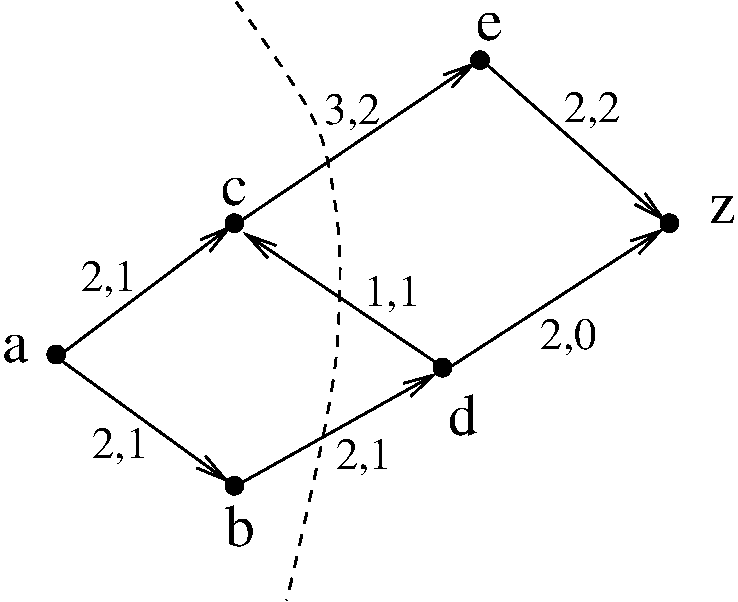
\includegraphics[width=0.3\linewidth,keepaspectratio]{snede1} % ,height=4cm}
\end{center}
\caption{A network with a flow and a cut\label{snede1}}
\end{figure}

We can check how much of the flow traverses the cut, i.e. from left to
right in the figure. While doing that, an edge from $P$ to
$\overline{P}$ should be counted as contributing to that quantity,
while the flow of the other edges must be subtracted. For the network
in Figure~\ref{snede1} we get: \mbox{$~~~~~~~~F(c,e) + F(b,d) -
F(d,c) = 2+1-1=2$ }

Comparing this number with the flow (in {\em a} or {\em z}), we notice
that these are also equal to 2! Coincidence?

We can also try to make an optimistic estimate of how much flow there
could maximally be over a cut: maybe there exists a flow that uses all
the capacity of the edges from $P$ to $\overline{P}$, and nothing is
flowing back over the other edges. We name this quantity the {\em
capacity of the cut}. In the example, we get \mbox{$~~~~~~~~C_{c,e} +
C_{b,d} = 2+3=5$}

The capacity of a cut seems larger than the flow over the cut, and
larger than the maximal flow (you can check that the maximal flow in
the example is 4). Is this a coincidence? We study this more formally.


 \begin{definition}[Capacity $C(P,\overline{P})$ of a cut]
  \textup{The \textbf{capacity of a cut} $(P,\overline{P})$ is
    $C(P,\overline{P}) = \displaystyle
    \sum_{i \in P} \sum_{j \in \overline{P}} C_{i,j}$}
\end{definition}

 \begin{theorem} \label{snedeflow}
The capacity of a cut is not smaller than a flow, i.e.
\[\sum_{i \in P} \sum_{j \in \overline{P}} C_{i,j} \geq \sum_{i \in V} F(a,i).\]
\end{theorem}
\begin{proof}
\begin{eqnarray*}
\sum_{i \in V} F(a,i) & = &
                \sum_{i \in V}(F(a,i) - F(i,a)) +
                \sum_{j \in P \backslash \{a\}} \sum_{i \in V}(F(j,i) - F(i,j))\\
        & = & \sum_{j \in P} \sum_{i \in V} (F(j,i) - F(i,j)) \\
        & = & \sum_{j \in P} \sum_{i \in P} F(j,i) +
                \sum_{j \in P} \sum_{i \in \overline{P}} F(j,i) -
                \sum_{j \in P} \sum_{i \in P} F(i,j) -
                \sum_{j \in P} \sum_{i \in \overline{P}} F(i,j)\\
        & = & \sum_{j \in P} \sum_{i \in \overline{P}} F(j,i) -
                \sum_{j \in P} \sum_{i \in \overline{P}} F(i,j)\\
        & \leq & \sum_{j \in P} \sum_{i \in \overline{P}} F(j,i)\\
        & \leq & C(P,\overline{P})
\end{eqnarray*}
\end{proof}

Note that from the last but two lines, you see that the flow equals
the flow over the cut.



A \textbf{minimal} cut is a cut with minimal capacity. The previous
theorem implies directly that any maximal flow is smaller than or
equal to the capacity of the minimal cut. The connection between the
two is even stronger:


 \begin{theorem}[Max flow - min cut \label{maxflowmincut}]
  Let $(P,\overline{P})$ be a cut and $F$ a flow in a network $G(V,E)$,
if
\[C(P,\overline{P})=F\mbox{ \ \ (or written out }
\sum_{i \in P} \sum_{j \in \overline{P}} C_{i,j} = \sum_{i \in V} F(a,i)
 \mbox{ )}\]
 then $F$ is maximal and the cut is minimal.\\
  Moreover, the equality is equivalent with
\begin{enumerate}
\item
$\forall i \in P, j \in \overline{P}: F(i,j) = C_{i,j}$ and
\item
$\forall i \in \overline{P}, j \in P: F(i,j) = 0$
\end{enumerate}
i.e. all good edges in the cut have a flow equal to their capacity and
all bad edges have zero flow.
\end{theorem}
\begin{proof}
All this follows from the inequalities in Theorem~\ref{snedeflow}
\end{proof}

Note that we have not proven that for each maximal flow there is a
minimal cut, neither the other way around.



Figure~\ref{snede2} shows a maximal flow with its minimal cut.

\begin{figure}[ht]
\begin{center}
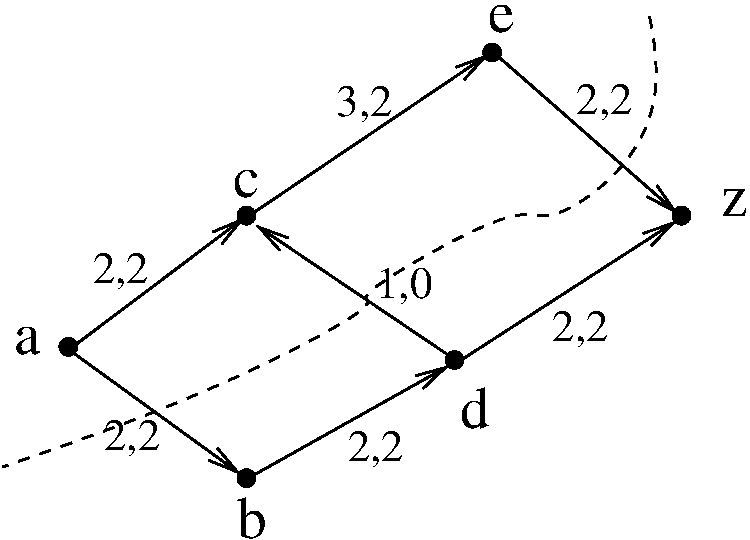
\includegraphics[width=0.35\linewidth,keepaspectratio]{snede2} % ,height=4cm}
\end{center}
\caption{A network with a maximal flow and its minimal cut\label{snede2}}
\end{figure}

We are now ready to prove that Algorithm~\ref{maxflow} ends with a
maximal flow.



\begin{proof} (of Algorithm~\ref{maxflow})\\
At the moment the algorithm ends, let $P$ be the set of vertices with
a label (note: $a \in P$) and $\overline{P}$ the set of vertices
without a label ($z \in \overline{P}$). $(P,\overline{P})$ is a cut.
Consider a (directed) edge $(i,j)$ with $i \in P$ and $j \in
\overline{P}$.  Since $i$ has a label $F(i,j)$ must be equal to
$C_{i,j}$, otherwise $j$ would have gotten a label. Now consider an
edge $(j,i)$ with $i \in P$ and $j \in \overline{P}$. Since $i$ has a
label, $F(j,i)$ must be equal to 0, otherwise $j$ would have gotten a
label. Together with Theorem~\ref{maxflowmincut}, we derive that $F$
is maximal.
\end{proof}

You see that the algorithm constructs a maximal flow
and a minimal cut at the same time. Some of the steps in Algorithm~\ref{maxflow} are
shown in Figure~\ref{maxflow1} and~\ref{maxflow2}:

\begin{figure}[ht]
\begin{center}
\subfigure[After initialisation and labeling source
a]{\includegraphics[width=0.4\linewidth,keepaspectratio]{maxflow1} \label{maxflow1}}
\hspace{1cm} \subfigure[After a labeling that reached
$z$]{\includegraphics[width=0.4\linewidth,keepaspectratio]{maxflow2} \label{maxflow2}}
\end{center}
\caption{Illustration 1 for Algorithm~\ref{maxflow}}
\end{figure}

Choose the order on the vertices as $(a,c,d,b,z)$. Starting from $a$,
$d$ and $b$ get a label. Then $c$ is labeled from $d$; $b$ is not
labeled from $d$ because $b$ has already a label. Then $z$ is labeled
from $c$: we have found a path from $a$ to $z$ as you can see in
Figure~\ref{maxflow2}. The flow is improved and the result is in
Figure~\ref{maxflow3}.

\begin{figure}[ht]
\begin{center}
\subfigure[After improving the flow the first
time]{\includegraphics[width=0.35\linewidth,keepaspectratio]{maxflow3} \label{maxflow3}}
\hspace{1cm} \subfigure[A second labeling has reached
$z$]{\includegraphics[width=0.35\linewidth,keepaspectratio]{maxflow4} \label{maxflow4}}
\end{center}
\caption{Illustration 2 for Algorithm~\ref{maxflow}}
\end{figure}

The labeling restarts in the situation of Figure~\ref{maxflow3}. From
$a$, $d$ is not labeled now: the flow on edge $(a,d)$ is already
maximal. $c$ does not get a label from $b$, because the edge $(c,b)$
is {\em bad} and its flow is zero, so it cannot be decreased. But $d$
gets a label from $b$, and since the capacity of edge $(b,d)$ (3)
is smaller than the $\Delta$ of $b$ (7 at that moment), we give $d$ a
$\Delta = 3$. $c$ gets a label from $d$ and since the unused capacity
$(d,c)$ equals 2, we give $c$ a $\Delta = 2$. From $c$, only $z$ can be
labeled: the resulting situation is in Figure \ref{maxflow4}. The flow
can be improved along the obtained path: the result is in
Figure~\ref{maxflow5}.

\begin{figure}[ht]
\begin{center}
\subfigure[After improving the flow for the second time]{\includegraphics[width=0.35\linewidth,keepaspectratio]{maxflow5} \label{maxflow5}} \hspace{1cm}
\subfigure[The labeling does not reach $z$: the cut is minimal, the
flow is
maximal]{\includegraphics[width=0.35\linewidth,keepaspectratio]{maxflow6} \label{maxflow6}}
\end{center}
\caption{Illustration 3 for Algorithm~\ref{maxflow}}
\end{figure}

At this moment, the flow is already maximal, but the algorithm has not
found that out: another attempt to construct a path from $a$ to $z$ is
needed. The last round of labeling start in the situation in Figure
\ref{maxflow5}: from $a$ we can label $b$ (the capacity of the edge
$(a,d)$ is already fully used) and also edge $(b,d)$ has some spare
capacity, but then we are stuck: the labeling stops at
Figure~\ref{maxflow6}. The minimal cut is defined by $P = \{a,b,d\}$ and
$\overline{P} = \{c,z\}$.

Run the algorithm (manually) for the networks in in
Figure~\ref{maxflow7}, with order $(a,b,c,d,e,z)$ on the vertices.

\begin{figure}[ht]
\begin{center}
\includegraphics[width=0.6\linewidth,keepaspectratio]{maxflow7} % ,height=3.2cm}
\end{center}
\caption{Two networks for practising \label{maxflow7}}
\end{figure}

Finding the maximal flow in a network is equivalent to finding
(integer) values $F(i,j)$ so that
\begin{itemize}
\item
$\sum_{j} F(a,j)$ is maximal
\item
$0 \leq F(i,j) \leq C_{i,j}$ for the given $C_{i,j}$
\item
$\forall j: \sum_{i} F(i,j) = \sum_{i} F(j,i)$
\end{itemize}

This type of problem can also be solved by linear programming,
e.g. by the simplex algorithm.

%===============================================================================
\section{Matching}

Consider the following problem: 4 students ($A,B,C$ and $D$) want to
make a separate appointment with an assistant who is available on 5
different days $(a,b,c,d$ and $e)$. Each student has their own
preference for one or more of the days. The assistant must now decide
who comes when.  Clearly, this is not always possible: e.g. if both
$A$ and $B$ have as their only preference day $a$, then it is
impossible. Even if it is possible, it is not trivial to solve such a
problem, especially not when there are many more students and days
involved.

At first sight, this problem is unrelated to graphs, but we can
represent it as a graph $G$ and work from there: the students and the
days play the role of the vertices of $G$. We draw a directed edge
between a student and a day, if that student has included that day in
their preference list. As an example: $A$ prefers $\{b,c\}$, $B$
prefers $\{a,b\}$, $C \{d,e\}$ and $D$ $\{b,c,e\}$. We get the graph
in Figure~\ref{matching1}

\begin{figure}[ht]
\begin{center}
\includegraphics[width=0.17\linewidth,keepaspectratio]{matching1} % ,height=4cm}
\end{center}
\caption{The graph for the matching problem\label{matching1}}
\end{figure}

This graph is bipartite and directed. The connection with the previous
section becomes clear if we add a source and a sink, and give each
edge 1 as capacity: see Figure~\ref{matching2}.

\begin{figure}[ht]
\begin{center}
\includegraphics[width=0.5\linewidth,keepaspectratio]{matching2eng} % ,height=4cm}
\end{center}
\caption{Network for the matching problem: all edges have capacity =
1\label{matching2}}
\end{figure}

We can now construct a maximal (integer) flow $F$ in in this network:
the value of this maximal flow is 4 (the number of students). We can
derive an assignment of students to days (or a matching of the
students with the days) by interpreting an edge $(s,d)$ so that
$F((s,d)) = 1$ as: student $s$ can see the assistant on day
$d$. Figure~\ref{matching3} shows a maximal flow with dotted lines. From this, we
can read out the assignment $(A,b)$, $(B,a)$, $(C,d)$,
$(D,e)$. The assignment is complete, and we have a complete (or
perfect) matching, since every student is matched up with a day.

\begin{figure}[ht]
\begin{center}
\includegraphics[width=0.5\linewidth,keepaspectratio]{matching3eng} % ,height=4cm}
\end{center}
\caption{A solution for the assignment problem\label{matching3}}
\end{figure}

The maximal flow could have been smaller than the number of
students (for a different set of preferences of course): that maximal
flow gives us a maximal matching, but not a complete one. More
formally:


 \begin{definition}
{\rm Let $G(V \cup W,E)$ be a directed, bipartite graph $G(V \cup
W,E)$ with $V \cap W = \emptyset$ and $E \subseteq V \times W$, then
$M$ is a \textbf{matching} if
\begin{verse}
\hspace*{1ex}$\bullet$
$M \subseteq E$ and

\hspace*{1ex}$\bullet$
$\forall (x,y),\;(i,j) \in M:$ if $(i,j) \neq (x,y)$ then
$i \neq x$ and $j \neq y$
(i.e. at most one edge arrives and leaves any vertex)
\end{verse}
A \textbf{maximal} matching has a maximal number of edges in $M$. A
matching is \textbf{complete} if $\forall v \in V,\; \exists w\in W:\;
(v,w) \in M$.  }
\end{definition}

A directed, bipartite graph $G(V \cup W,E)$ to which a source and sink
are added, with edges from the source to all the vertices in $V$, and edges from
all the vertices in $W$ to the sink, with a capacity of 1 for every
edge is named the \textbf{matching network} derived from $G$.


The next theorem formalises the correspondence between a maximal
flow in a matching network and a maximal matching.

 \begin{theorem}
Let $G(V \cup W,E)$ be a directed, bipartite graph
with $V \cap W = \emptyset$ and $E \subseteq V \times W$, then the
following is true:
\begin{verse}
\hspace*{1ex}$\bullet$
An integer flow in the corresponding matching network $F$ gives a
matching in $G$: $v \in V$ corresponds to $w \in W$ if and only if
$F(v,w) = 1$

\hspace*{1ex}$\bullet$
A maximal integer flow corresponds to a maximal matching.

\hspace*{1ex}$\bullet$
An integer flow with value $\#V$ corresponds to a perfect matching.
\end{verse}
\end{theorem}
\begin{proof}
You can work out the proof yourself.
\end{proof}

It is sometimes possible to quickly test that no perfect matching
exists: clearly, when $n$ students together prefer strictly fewer than
$n$ days, they cannot all get one of their preferred days. We generalize this:

\begin{itemize}
\item
define the mapping \footnote{${\cal P}(S)$ denotes the power set of
$S$}

\begin{center}
$
\begin{array}{lrcl}
R: & {\cal P}(V) & \rightarrow & {\cal P}(W)\\
   & S    & \mapsto     &
                \{w\in W \;|\; \exists v \in S \mbox{ with }(v,w) \in E\}
\end{array}
$
\end{center}
\item
If $G$ has a perfect match, then $\#S \leq \#R(S)$ holds $\forall S
\subseteq V$
\end{itemize}

The English mathematician Philip Hall proved the converse in 1935:
\begin{theorem}[Hall's marriage theorem] \label{hall}
A directed, bipartite graph $G(V \cup W,E)$ with $V \cap W =
\emptyset$ and $E \subseteq V \times W$, has a perfect match if and
only if $\#S \leq \#R(S),\; \forall S \subseteq V$
\end{theorem}
\begin{proof}~
\begin{itemize}
\item[\fbox{$\Rightarrow$}]
We have already argued this.
\item[\fbox{$\Leftarrow$}]
Let $m = \#V$. We prove this direction by induction on $m$.
\begin{itemize}
\item[\underline{$m=0$}:] Then the perfect match is trivial: $M = \emptyset$.
\item[\underline{$m>1$}:] 
We distinguish two mutually exclusive cases: whether or not 
for all $S$ such that $\emptyset \neq S \subsetneq V$ it
is true that $\#S \leq \#R(S) - 1$.
\begin{itemize}
\item[\dashuline{$\forall S: \emptyset \neq S \subsetneq V \Rightarrow \#S \leq
\#R(S) - 1$:}] Take any edge $(v,w) \in G$ and construct the bipartite graph
$G' = G \setminus \{v,w\}$. Hence the vertex partitions of $G'$ are $V
\setminus \{v\}$ and $W \setminus \{w\}$. So $m' = \#(V \setminus \{v\}) = m - 1 < m$.
Clearly, $G'$ poses a smaller problem than $G$. Now let us show that it satisfies
the condition of Hall's Theorem.
\begin{itemize}
\item[]
Before we proceed, from now on we add a subscript to $R$ with the target vertex
set to avoid confusion between $G$ and $G'$. 

It follows from the definition of $R$ that 
\[ \forall T \subseteq V: R_{W \setminus \{w\}}(T) = R_W(T) \setminus \{ w\}\] 
Moreover, for any two sets $A, B$, it is true that $\#A - \#B \leq \#(A
\setminus B)$. Hence, it follows that
\[ \forall T \subseteq V:  \#R_W(T) - 1 \leq \#R_{W \setminus \{w\}}(T)\] 

Now let us restate the case assumption:
\[\forall S: \emptyset \neq S \subsetneq V \Rightarrow \#S \leq \#R_W(S) - 1\]
As $V \setminus \{ v \} \subsetneq V$, it follows that:
\[\forall S: \emptyset \neq S \subseteq V\setminus \{ v \} \Rightarrow \#S \leq \#R_W(S) - 1\]
If we take the upper bound for $\#R_W(S) - 1$ into account:
\[\forall S: \emptyset \neq S \subseteq V\setminus \{ v \} \Rightarrow \#S \leq \#R_{W\setminus\{w\}}(S)\]
Because $R(\emptyset) = \emptyset$ in any bipartite graph, we can include $S = \emptyset$ in the above:
\[\forall S: S \subseteq V\setminus \{ v \} \Rightarrow \#S \leq \#R_{W\setminus\{w\}}(S)\]
\end{itemize}
This establishes the condition of Hall's Theorem for $G'$. Hence, we can apply the induction
hypothesis to $G'$ and conclude that $G'$ has a perfect match $M'$. We can extend
this perfect match for $G'$ to a perfect match for $G$ by adding the removed edge $(v,w)$:
$M = M' \cup \{ (v,w)\}$.
 
\item[\dashuline{$\exists S: \emptyset \neq S \subsetneq V \wedge \#S =\#R(S)$:}]
In this case we can partition $G$ into two bipartite subgraphs $G_1$ and $G_2$,
illustrated in Figure \ref{hallfig}. $G_1$ gets the vertex partitions $S$ and $R_W(S)$, 
while $G_2$ gets the remainders $V \setminus S$ and $W \setminus R_W(S)$.
If we can show that $G_1$ and $G_2$ are smaller and satisfy Hall's condition,
we can apply the induction hypothesis to them. It follows that $G_1$
has a perfect match $M_1$ and $G_2$ has a perfect match $M_2$. As $G_1$ 
and $G_2$ are disjoint, so are there matchings and together they
form a perfect match for $G$: $M = M_1 \cup M_2$.

All that remains is to show that $G_1$ and $G_2$ indeed satisfy the necessary
conditions.
\begin{itemize}
\item[\dotuline{$G_1$:}]
As $S$ is a strict subset of $V$, we have that $m_1 = \#S < \#V = m$.
So $G_1$ is indeed smaller.

Let us state upfront a property of $R$ that we will need shortly:
$R$ preserves the subset relation:
\[ \forall A, B. A \subseteq B \Rightarrow R(A) \subseteq R(B) \]
This follows trivally from the definition of $R$.

Let us formulate again the assumption that Hall's condition applies to $G$:
\[ \forall T \subseteq V: \#T \leq \#R_W(T) \]
Because $S \subsetneq V$:
\[ \forall T \subseteq S: \#T \leq \#R_W(T) \]
Also, because $R$ preserves the subset relation, 
we know that $R_W(T) \cap R_W(S) = R_W(T)$. Hence,
\[ \forall T \subseteq S: \#T \leq \#(R_W(T) \cap R_W(S)) \]
Moreover, because $R_W(S) \subseteq W$, we have that
\[ \forall T \subseteq S: \#T \leq \#R_{R_W(S)}(T) \]

In other words $G_1$ satifies both conditions of
the induction hypothesis.

\item[\dotuline{$G_2$:}]
As $V$ is non-empty and $S$ is a non-empty subset of $V$, we have that $m_2 =
\#(V \setminus S) < \#V = m$. So $G_2$ is indeed smaller.

Let us formulate yet again the assumption that Hall's condition applies to $G$:
\[ \forall T \subseteq V: \#T \leq \#R_W(T) \]
Since $\forall T \subseteq V\setminus S: T \cup S$, we can specialize this to:
\[ \forall T \subseteq V \setminus S: \#(T \cup S) \leq \#R_W(T \cup S) \]
Because $T$ and $S$ are disjoint, we have that $\#(T \cup S) = \#T + \#S$:
\[ \forall T \subseteq V \setminus S: \#T + \#S \leq \#R_W(T \cup S) \]
Also, as $R$ preserves union, we have that $R_W(T \cup S) = R_W(T) \cup R_W(S)$:
\[ \forall T \subseteq V \setminus S: \#T + \#S \leq \#(R_W(T) \cup R_W(S)) \]
We also have for all sets $A, B$ that $\#(A \cup B) = \#A + \#B - \#(A \cap B)$.
So:
\[ \forall T \subseteq V \setminus S: \#T + \#S \leq \#R_W(T) + \#R_W(S) - \#(R_W(T) \cap R_W(S)) \]
Since we have assumed that $\#S = \#R_W(S)$, we can simplify this to:
\[ \forall T \subseteq V \setminus S: \#T \leq \#R_W(T) - \#(R_W(T) \cap R_W(S)) \]
As before, we can rewrite the last term:
\[ \forall T \subseteq V \setminus S: \#T \leq \#R_W(T) - \#R_{R_W(S)}(T) \]
Finally, we can also rewrite the right-hand side:
\[ \forall T \subseteq V \setminus S: \#T \leq \#R_{W \setminus R_W(S)}(T) \]

In other words $G_2$ satifies both conditions of
the induction hypothesis.

\end{itemize}
\end{itemize}
\end{itemize}

\end{itemize}
\end{proof}

\begin{figure}[h]
\begin{center}
\includegraphics[height=0.35\textheight,keepaspectratio]{hall}
\caption{The dashed lines belong to the original graph, but not to $G_1$ and $G_2$}\label{hallfig}
\end{center}
\end{figure}

Hall's Theorem~\ref{hall} can be used in partner choice problems, hence its name.



% http://myweb.facstaff.wwu.edu/sarkara/hall.pdf geeft een mooier bewijs
% van de stelling van Hall, eentje waarvoor geen kennis van networken
% nodig is.




